% Tipo di documento. L'uso di twoside implica che i capitoli inizino sempre con la prima pagina a sinistra, eventualmente lasciando una pagina vuota nel capitolo precedente. Se questa cosa è fastidiosa, è possibile rimuoverlo. 
% \documentclass[a4paper, twoside,openright]{report}
\documentclass[a4paper,openright]{report}

\usepackage{graphicx} % Required for inserting images
\setkeys{Gin}{width=0.6\textwidth}

\usepackage[utf8]{inputenc}

\usepackage{hyperref}

\usepackage{graphicx}
\usepackage{wrapfig}

\usepackage{enumitem}
\setitemize{noitemsep}
\setenumerate{noitemsep}
\setlist{noitemsep}

\usepackage{paracol}
\usepackage{multicol}

\usepackage{geometry}

\usepackage{color}

\usepackage{listings}

\usepackage{amsmath}
\usepackage{bm}

\usepackage{wasysym}

% Uso dei colori
\usepackage[dvipsnames]{xcolor}

\usepackage{tikz}
\usetikzlibrary{positioning}
\usetikzlibrary{shapes.geometric}
\usepackage{parskip}

\geometry{margin=0.6in}

\setlist[description]{itemsep=0em,topsep=0.5em,parsep=0em}
\setlist[itemize]{itemsep=0em}

\hypersetup{
    colorlinks=true,
    linkcolor=black,
    filecolor=mauve,
    urlcolor=blue,
}

\definecolor{gray}{gray}{0.3}

\newenvironment{notes}{
\par
\color{gray}
\small}

\newcommand{\note}[1]{\begin{notes}{#1}\end{notes}}
\newcommand{\nl}[0]{\parskip = \baselineskip}

\lstset{frame=false,
 showstringspaces=false,
 breaklines=true;
 columns=flexible,
 basicstyle={\small\ttfamily},
 keywordstyle=\color{blue},
 commentstyle=\color{dkgreen},
 stringstyle=\color{mauve}
 tabsize=3
}

\title{ICT Risk Assessment - Appunti}
\author{Francesco Lorenzoni}
\date{September 2023}

\begin{document}

\maketitle
\tableofcontents

\chapter{Introduction}
\section*{27 - Settembre}
\section{Product based}
In \textit{Project-based SE} there is loop which nowdays cripples software since its early stages of development.
This is due to mutable nature of requirements, which often change throughout time along the features implemented by the software.
\begin{center}
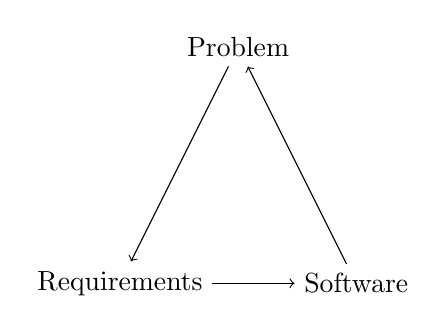
\begin{tikzpicture}
    \node[draw=white,align=left] (A) at (1.5,3) {Problem};
    \node[draw=white,align=left] (B) at (0,0) {Requirements};
    \node[draw=white,align=left] (C) at (3,0) {Software};

    \path [->] (A) edge node[left] {} (B);
    \path [->] (B) edge node[left] {} (C);    
    \path [->] (C) edge node[left] {} (A);    
\end{tikzpicture}
\end{center}

\textit{Product-based SE} is opposed to \textit{Project-based SE} and the above pictures changes as follows.

\begin{center}
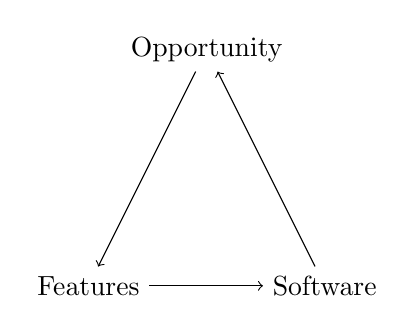
\begin{tikzpicture}
    \node[draw=white,align=left] (A) at (1.5,3) {Opportunity};
    \node[draw=white,align=left] (B) at (0,0) {Features};
    \node[draw=white,align=left] (C) at (3,0) {Software};

    \path [->] (A) edge node[left] {} (B);
    \path [->] (B) edge node[left] {} (C);    
    \path [->] (C) edge node[left] {} (A);    
\end{tikzpicture}
\end{center}

\section{Agile}
Agile is a collection of principles and methods applied in the software development field.
\nl

Opposed to project-based SE, in Agile the client is requested to express the requirements not in technical terms but in features.

Agile suggests an incremental development model

\subsection*{Principles}
\begin{enumerate}
    \label{subsec:agile_principles}
    \item Satisfy customer through early and continuous delivery of valuable software
    \item Welcome changing requirement, even late in development.
    Agile processes harness change for the customer's comptetitive advantage
    \item Deliver working software frequently, from a couple of weeks to a couple of months, with a preference to the shorter timescale
    \item Business people and devs must work together daily throughout the prokect
    \item Build porjects around motivated individuals and give them the environment and support they need
    \item The most efficient and effective method of conveying information to and within a dev team is face-to-face conversation
    \item Working software is the primary measure of progress
    \item Agile processes promote sustainable dev 
    \item Continuous attention to technical excellence and good design enhances agility
    \item Simplicity i.e. art of maximizing the amount of work not done is essential
    \item The best architectures, requirements, and designs emerge from self-organizing teams.
\end{enumerate}

Extreme Programming was proposed as part of the agile methodology

\section{Scrum}
Since requirements changes are rather frequent, long-term plans are unreliable,
hence SE aims to formulate short-term plans.

Scrum is found on \textbf{empiricism} and \textbf{lean thinking}; it asserts that knowledge comes from experience, and that decisions should be made on observations.

Other key terms are code \textbf{Transparency} among the team and with the customer, \textbf{Inspection} of produced code and software (artifacts), \textbf{Adaptation} to changes in features and requirements.

The \textbf{Scrum Team} is composed by:
\begin{enumerate}
    \item \textbf{Product Owner}: must ensure that the dev team is always focused on the goal
    \item \textbf{Scrum Master}: Scrum expert which drives the team to apply properly the Scrum framework.
    \item \textbf{Developers}: actual monkeys people which write code
\end{enumerate}

In scrum SW is developed in \textbf{sprints}, i.e. fixed-length periods with a specific goal to be achieved.

\begin{itemize}
    \item Product backlog: to-do list of items to be implemented
    \item Timeboxed sprints
    \item Self-organizing teams
\end{itemize}

...
\textbf{Prod Backlog Revised}\\
\textbf{PBI Estimation Metrics}

\subsection{Timeboxed Sprints}
Even if at the end of a srpint the goal hasn't been reached, "no worries", the work stops anyway;
there will be a new sprint which will include the work which has not been implemented in the previous one.

\subsection{Scrum Meetings}

\subsection{Agile activities}
Test automation
Continuous integration

\subsection{Sprint reviews}
At the end of each sprint there is a review meeting which involves the \textit{whole} team.
The \textit{product owner} has the ultimate authority to decide wether the sprint goal has been reached or not.
The sprint review should include a process review, in which the whole team shares ideas on how to improve their way of working.

\textbf{Team size}\nl

\section{5 - Ottobre}



\chapter{IEEE 802.11}

\begin{figure}[htbp]
   \centering
   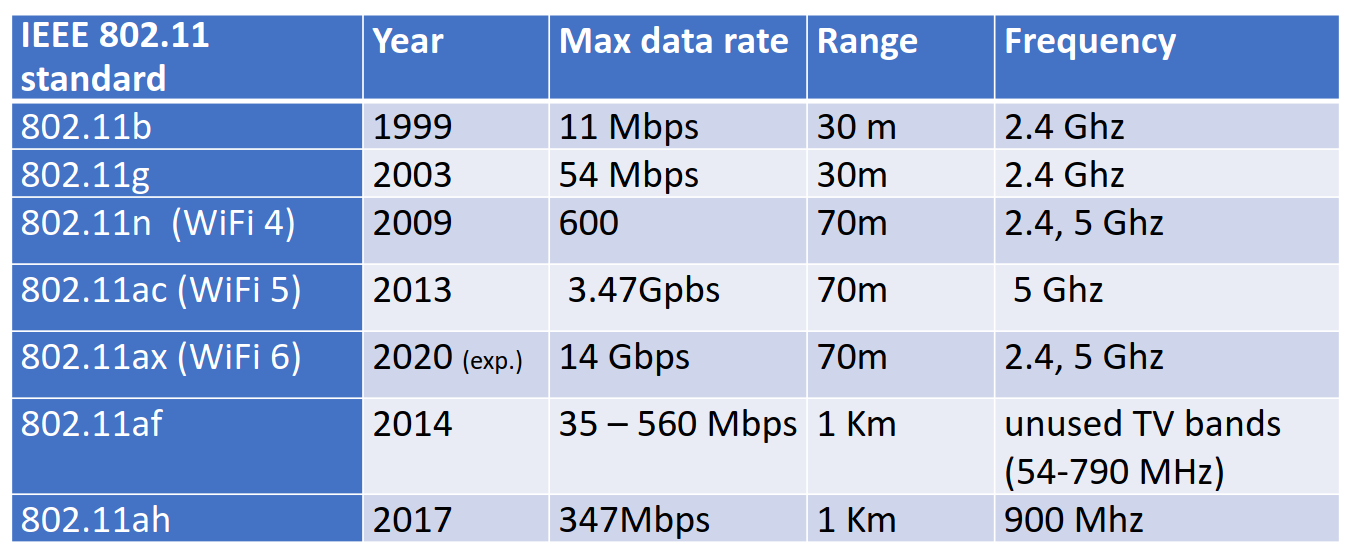
\includegraphics{images/ieee_bgn.png}
   \caption{IEEE 802.11 standards}
   \label{fig:ieee_bgn}
   All these standards \texttt{use \texttt{CSMA/CA} for multiple access}, and have base-station and ad-hoc network versions
\end{figure}

IEEE 802.11 standards refer to the \textit{Physical} Layer.
In case of an AP (Access Point), every station must channel its communication through the AP to talk to any other. Otherwise, in an \textit{Ad-Hoc} network, stations can communicate directly with each other.

TODO

\note{TODO non ci sono domande su questa cose nel pdf}
\chapter{Fabric}
``Fabric'' is the term used to refer to the \textit{interconnection} between nodes of a datacenter.\\
\ul{Cabling is of paramount importance.}
\note{Prof. Cisternino learnt it ``the hard way'' when he performed the cabling of the first UniPi datacenter by himself}
\begin{enumerate}
   \item Maintenance
   \item Cooling
   \begin{enumerate}
      \item Cables may heat up
      \item Cables may obstruct air flow
   \end{enumerate}
   \item Determines which machines interact with each other (\textit{fabric})
   \item Bandwidth
   \item Not neglectable cost
\end{enumerate}

We refer to North-South traffic indicating the traffic outgoing and incoming to the datacenter (internet), while we refer to East-West as the internal traffic between servers.
Most of the network (or fabric) traffic is processed horizontally (North-South traffic)\footnote{Seems odd that ``horizontal'' refers to North-South traffic, but that's how it is.}.


\section{Bandwidth and Storage implications}
\label{sec:bandwidth_storage}
A standard datacenter has servers connected with 25Gbit links in both directions, summing up to 50Gbit total bandwidth.
Current SSDs using NVMe provide much more, about $3.5 GB/s$, making \ul{4 drives are enough to saturate a 100Gbit/s link.}\\
We moved from a situation where the \textbf{bottleneck} were slow Hard Drives, to the current one where the bottleneck is the ---network--- \textbf{bandwidth}.\\
Recently the PCI 3.0, which lasted very long ---providing roughly$\sim\texttt{120Gbit/s}$ using 16 pin---, suddenly become unsufficient to handle the needed traffic.

Considering this, \ul{datacenters must be designed to allow \textit{Terabytes} of data to be moved in east-west traffic.}

\begin{center}
   \ul{\textit{The \textbf{fabric} is the glue that makes the datacenter possible.}}
\end{center}

Besides, a single server is \textit{unable} to handle 10TBs of data and handling requests from 3000 users simultaneously. It is necessary to \textbf{distribute} the requests.

HDDs are still currently used for \textbf{cold storage};
CPUs will access data exclusively from SSDs, and sometimes the server is shipped with on board \textbf{full-flash storage}.\\
The difference in price between SSDs and HDDs becomes negligible since you pay for top CPU, top GPU, top RAM;
furthermore, you can't waste ---the high amount of--- energy ---consumed by such components--- by waiting for a slow drive.

SSDs have a known write limit, but today, the usually last enough time: if you write the whole disk every day it will last for 5 years. Most-likely after five years you'd have to renew some components anyway, besides the failure is a predictable event.

\section{Cables and standards}
\subsection{Optical}
Electric current propagates at a speed $s = {\sim}0.6c$.
Hence \textbf{optical fiber} is ---at least in theory?--- faster.

\textbf{Lasers} are a coherent beam of equal fotons. It is possible to transfer energy through such fotons. Something resembling a laser is used for optical fibers.

Blu-Ray came out when scientists managed to create light using frequencies in the Blu area, which are the higher ones.
Currently, the best and most expensive optical fibers exploit blu-lasers as source of light.

Note that with optical you always need 2 fibers, one sending and the other receiving. The two possible connectors are \texttt{SC} and \texttt{LC}.
Sometimes the two ends of the cable are detachable so that the cables may be switched; this is useful because sometimes you may want to attach the TX cable on the RX plug and viceversa. 

\begin{figure}[htbp]
   \centering
   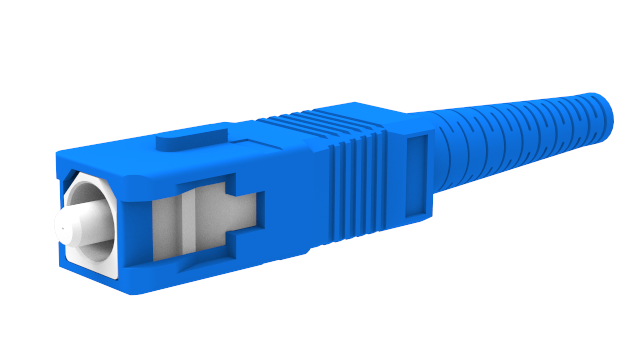
\includegraphics[width=0.25\columnwidth]{images/SC.png}
   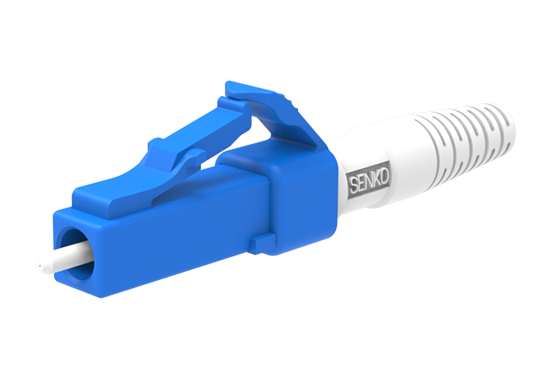
\includegraphics[width=0.25\columnwidth]{images/LC.png}
   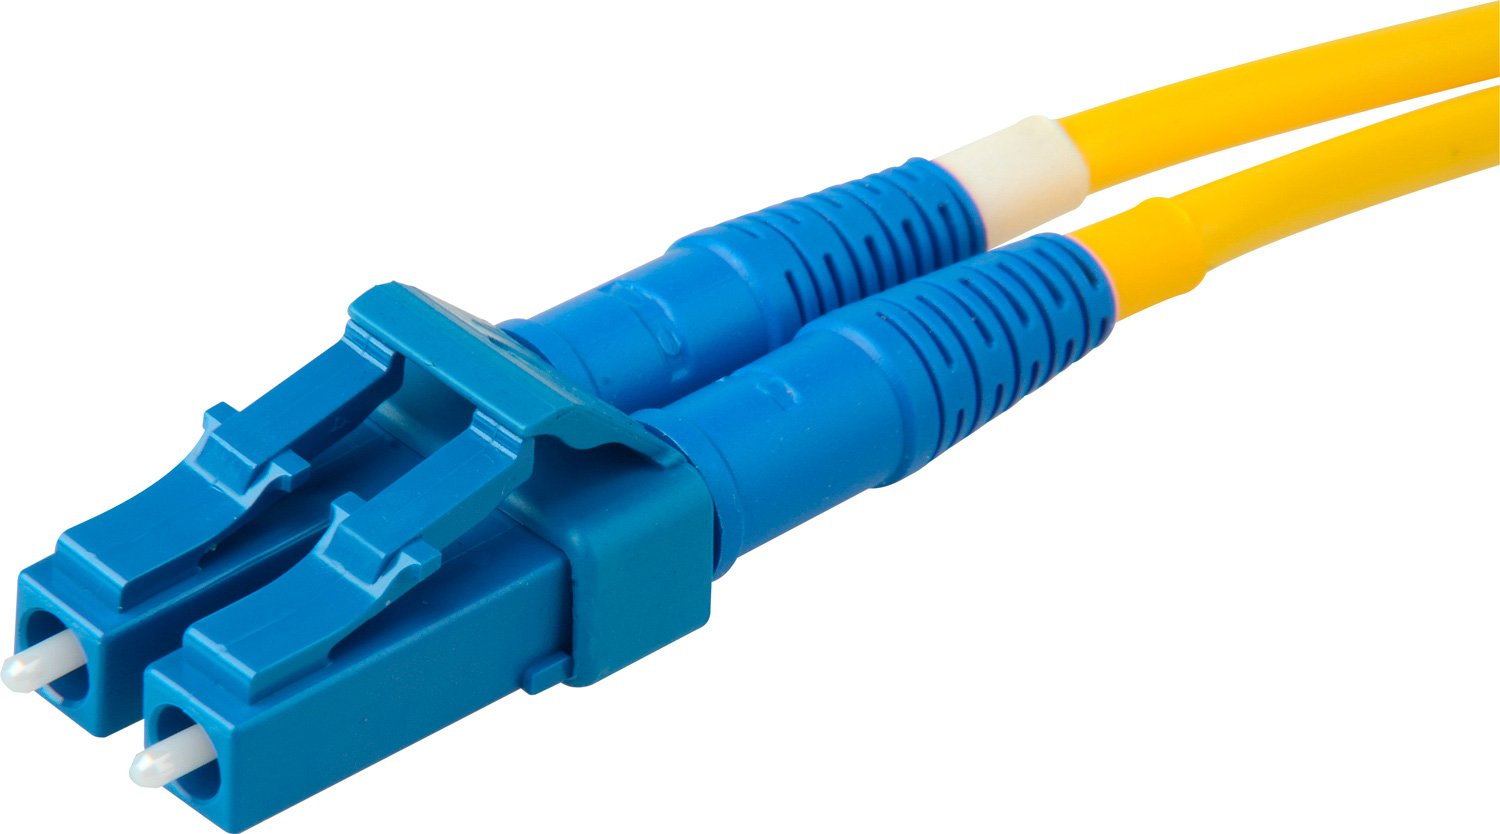
\includegraphics[width=0.25\columnwidth]{images/LC_coupled.JPG}
   \caption{\texttt{SC} and \texttt{LC} connectors}
   \label{fig:sc_lc_connectors}
\end{figure}

\subsection{Copper wires}
In case of electricity there are many aspects to be considered. Interferences, cable diameter/size, length, and also the fact that if a \texttt{1} has been transmitted for some time, it takes longer to transmit a \texttt{0}, due to the \textit{commutation} that must happen.
\nl

\begin{paracol}{2}
   \colfill
   \textbf{RJ45} is a standard physical interfaced for copper wires, which allows up to 1Gbit regularly.
   The \texttt{Cat 7} cables still use the RJ45 as connector and provide instead 10Gbit/s, but are very uncomfortable, they are so thick that they are difficult to bend.
   
   It is estimated that there have been installed $70 \times 10^9m$ of Ethernet cables, making them the most used.
   \colfill
   \switchcolumn

   \begin{figure}[htbp]
      \centering
      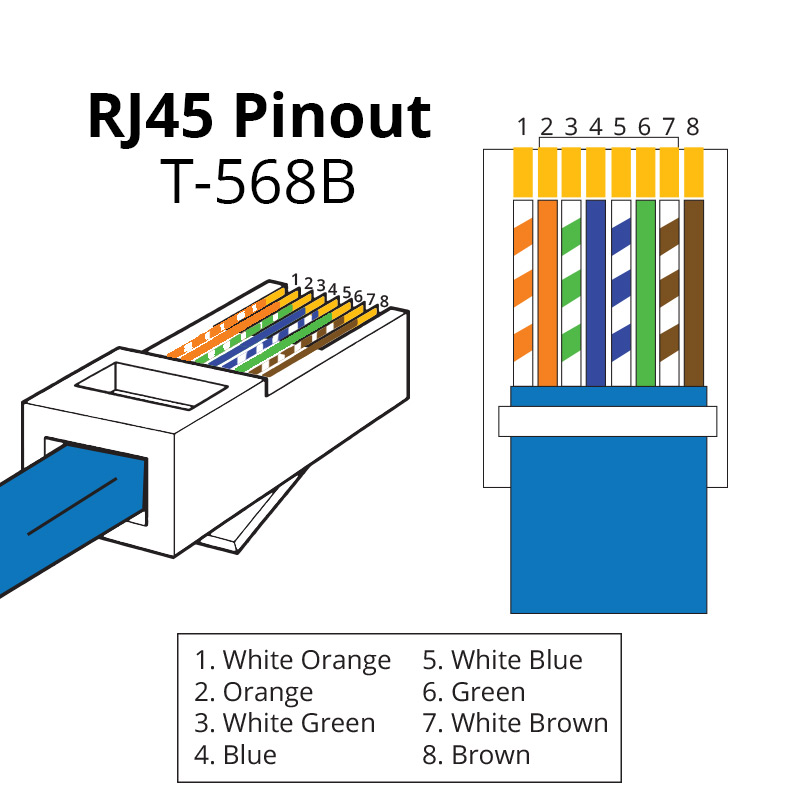
\includegraphics{images/RJ45_T568B.jpg}
      \caption{RJ45 - T568B}
      \label{fig:RJ45_T568B}
   \end{figure}
\end{paracol}

\subsection{SFP - Small Form-factor Pluggable}
There can be a cable with a LC in one side and a SC on the other side.
Instead of making switches with the optical plugs, switches were created with electrical plugs that would be able to host a \textbf{standard transceiver}.
The latter is a pluggable module that will receive current power and electrical signals for the transmission, which is responsible for transitioning between electrical signals and Optical signal (and viceversa).

\begin{paracol}{2}
   
   The aim of SFP is to decouple the optical transceivers from the server modules.
   \note{Is this correct?}
   They allow to go \textit{optic-copper}, \textit{copper-optic}, \textit{optic-optic} and \textit{copper-copper}.\\
   SFP and GBIC (oldest one, now dead) pluggable modules acting as active transceivers for optical wiring using RJ45 connector.\\
   \ul{A single cable having SFP ends costs about 100€}.
   The cost ain't neglectable \smiley.
   \note{\begin{itemize}
      \item[\texttt{SFP}] $\longrightarrow 1Gbit $
      \item[\texttt{SFP+}] $\longrightarrow 10Gbit $
      \item[\texttt{SFP28}] $\longrightarrow 25Gbit$
      \note{This is the current standard}
      \item[\texttt{QSFP28}] $\longrightarrow 4\times25Gbit$
   \end{itemize}}


   \switchcolumn

   \begin{figure}[htbp]
      \centering
      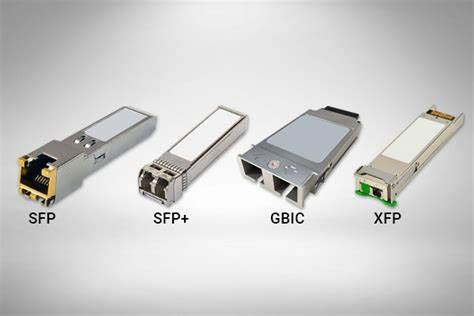
\includegraphics{images/sfp.jpeg}
      \caption{SFP transceivers form factors}
      \label{fig:sfp}
   \end{figure}
\end{paracol}

\note{Fun fact: ci sono 9 cavi USB-C e solo due portano informazioni video.}

\subsubsection{Issues about cabling and fabric}
The key point is that it would be desirable for cabling to be reconfigurable, that's why transceivers are so important.

\note{There are things called \textit{``Muffole''}, which are used for joining optical fiber cables, allowing for longer distances to be covered.
They are designed to be underground.}

Data traffic is always at least SFP+.
Current standard is SFP28. Various SFP are typically compatible, the shape of the plug should stay the same.
On switches there also some ports which are \texttt{QSFP+} or \texttt{QSFP28}, which allow up to \texttt{40} and \texttt{100Gbit/s} respecitively, and are used for north-south traffic.
\note{The \texttt{Q} letter stands for \textit{Quality}}

Switches for datacenters should be \textbf{non-blocking}, meaning that no port has to wait for other ones ---or any other thing--- before transmitting, they can also transmit simultaneously.


\ul{In every datacenter it is \textit{MANDATORY} to document the cabling.}

\subsection{InfiniBand}
Even though Ethernet is famous, it is not the only standard. InfiniBand is another one, which is used in supercomputers and known for its very high throughput and very low latency ($\sim 2\mu s$).
It may send messages up to 2GB each, with 16 priority levels.
It is a \textit{lossless protocol}, meaning that if a packet is received, its integrity is guaranteed.

\textit{IB} avoids TCP/IP stack, which is very heavy, and instead uses MPI (\textit{Message Passing Interface}), which is a way to distributed parallel programs, also exploited by OmniPath.

InfiniBand cables and connectors look similar to Ethernet ones, but they are not compatible.

Aside from HPC environments, it is uncommon to build an entire network with InfiniBand, typically there is an IB switch to whom the servers equipped with IB NICs are connected, which intereacts with the rest of the network with Ethernet, because ``it's cheaper and it works''.
\note{Today, we are about 400 Gbit/s on both IB and Ethernet.}

\subsection{RDMA - Remote Direct Memory Access}

RDMA is a technology API based (not a protocol!) that allows to access memory of a remote machine without involving the CPU or the OS of the remote machine.

RDMA supports zero-copy networking by enabling the network adapter to transfer data directly to or from application memory, eliminating the need to copy data between application memory and the data buffers in the operating system.\\
The main use case is distributed storage.

RoCE (\textit{RDMA over Converged Ethernet}) is a network protocol that allows remote direct memory access (RDMA) over an Ethernet network.

\subsection{Omni-Path}
Omni-Path is a high-performance computing network architecture, developed by Intel. It is a successor to Intel's InfiniBand, and competes with InfiniBand's EDR and HDR technologies.

Intel plans to develop technology that will serve as the on-ramp to \textit{exascale computing}\footnote{A computing system capable of the least one exaFLOPS}, which is the next frontier in high-performance computing.


\chapter{BitTorrent}

The goal of \textit{Content Distribution Networks} is to distribute web contents to hundreds of thousands or millions
of simultaneous users, \ul{exploiting data and/or service \textbf{replication} on different \textbf{mirror servers}}.

In \textbf{P2P CDN} the initial file request are served by a centralized server, and further requests served by peers which have already received and replicated the files (\textbf{\textit{seeders}}), without involving the initial server.

\begin{center}
\fbox{
   \begin{minipage}{0.8\columnwidth}
      \nl
      \begin{center}
         \ul{\textbf{BitTorrent} in a nutshell}
      \end{center}
      \nl

      \begin{itemize}
         \item Basically a \textit{Content Distribution Network} (\texttt{CDN})
         \item A distributed set of hosts cooperating to distribute large data set to end users.
         \item Efficient content distribution systems using \textit{file swarming}
         \item Does \textit{not} perform all the functions of a typical P2P system, like searching
         \item Rather than providing a search protocol itself, was designed to integrate seamlessly with the Web and made file descriptors available via Web, which could be searched with standard Web search
         \item \textit{File swarming}: a peer makes whatever portion of the file that is downloaded immediately available for sharing
      \end{itemize}
   \end{minipage}  
   }
\end{center}

\section{Deeper into BitTorrent}
\begin{figure}[htbp]
   \centering
   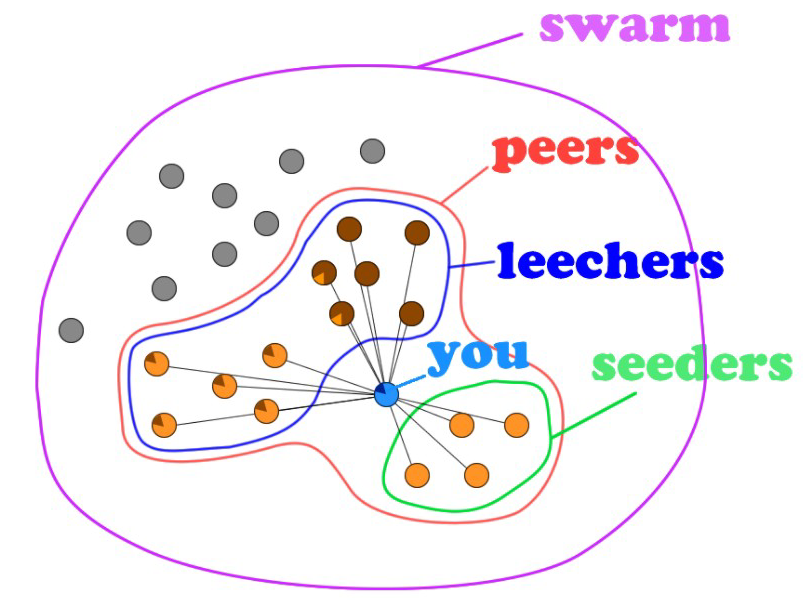
\includegraphics{images/bit_swarmschema.png}
   \caption{Swarm schema}
   \label{fig:bit_swarmschema}
\end{figure}
\subsection{Glossary}
\begin{itemize}
   \item \textbf{tracker}: active entity which coordinates
   the peers sharing the file, taking trace of who is currently providing the content
   \note{\begin{itemize}
      \item Joe connects to the tracker announcing the content
      \item the tracker now knows Joe is providing the file
   \end{itemize}}
   \item \texttt{.torrent} a descriptor of the file to be published on a server, which includes a reference to a tracker
   \item \textbf{swarm} set of peers collaborating to the distribution of the same file coordinated by the same tracker
   \item \textbf{seeder} peer which owns all the parts of the file
   \item \textbf{leecher} peer which has some part or no part of the file and downloads the file from the seeders and/or from other lechers.
\end{itemize}

\subsection{Protocol Overview}
\begin{figure}[htbp]
   \centering
   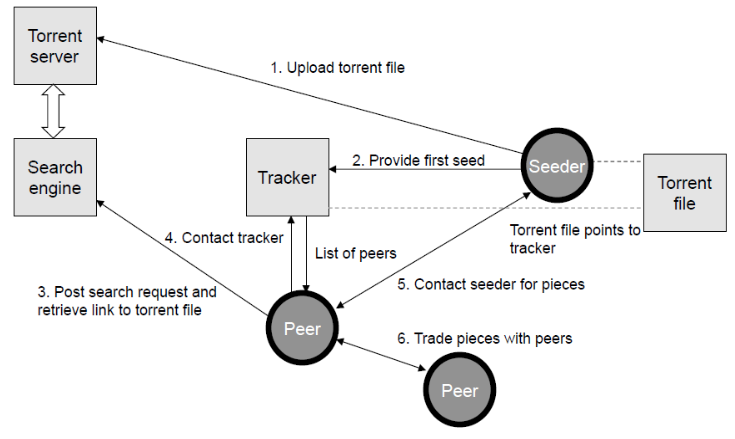
\includegraphics{images/bit_overview.png}
   \caption{BitTorrent protocol overview}
   \label{fig:bit_overview}
   BitTorrent protocol is built on top of HTTP
\end{figure}
\labelitemize{\textit{Seeder}}{
   \begin{enumerate}
      \item Upload the .torrent on a Torrent Server
      \item Opens a connection to the Tracker and informs it of its own existence: for the moment, it is the only peer which owns the file
   \end{enumerate}
}
\labelitemize{\textit{Peers}}{
   \begin{enumerate}
      \setcounter{enumi}{2}
      \item Retrieves the file descriptor (.torrent) and opens it through the BitTorrent
      client
      \item Opens a connection to the tracker and informs it of its own existence and
      receives from the tracker a list of peers of the swarm
      \item Opens a set of connections with other peers of the swarm.
   \end{enumerate}
}

Objects are serialized in \textbf{Bencode}, which is ---not popular as \texttt{JSON}--- used only in torrent; provides 4 data types: String, Integer, Lists and Dictionaries.\\
Content is split into chunks called pieces (256KB - 2MB):
when a peer receives a piece, it becomes the seeder of that piece.
\note{
   \ns
      There is a SHA-1 hash per piece stored in the .torrent file, used to check the piece once it is fully downloaded, 
      allowing to require retransmission in case the check fails.\\
      Pieces size got adapted to have a reasonably small .torrent file
}
Pieces are then split in \textbf{subpieces} (\textit{\textbf{blocks}}) of 16KB, with each one downloadable from a different peer, optimizing the bandwith and allowing \textit{pipelining}, decreasing the overall download time.

Trackers keep a database of swarms identified by torrent hash, and knows also the state of each peer in each swarm.
In the last versions, \textbf{trackerless} BitTorrent uses \textit{Kademlia DHT} to avoid the centralization point of the tracker.

\section{Pieces selection}
The order in which pieces are selected by different peers is critical for good performance, to avoid making peers end up stuck with the same pieces.
\labelitemize{\textit{Policies}}{
   \begin{itemize}
      \item \textbf{Strict Priority}\\
      Complete the ``assembling'' of a piece before asking for another piece
      \item \textbf{Rarest First}\\
      Download the rarest pieces first
      \item \textbf{Random First Piece}\\
      Choose a random piece ---only--- in the bootstrap phase
      \item \textbf{Endgame}\\
      When the file download is almost terminated, the remaining pieces are required in \textit{parallel} to all peers who own them.
      This policy is executed for a small period of time
   \end{itemize}
}

\subsection{Free Riders}
Free riders in BitTorrent are peers that do not put their bandwidth at disposal of the community.\\
Several non official BitTorrent clients enable the user to limit the upload bandwidth as they like.

However, an approach to solve this problem is based on \textbf{reciprocity}, allowing a client to obtain a good service if and only if it gives a good service to the community, by exploiting a dynamic strategy based on connection monitoring called ``Tit for Tat'', implemented using \textbf{choking}:\\
choking means \textit{temporarily} refusing to upload to another peer, but still downloading from them;  
the principle is to upload to peers who have uploaded to us.

\labelitemize{\textit{Choking}}{
\begin{center}
   \textit{The local peer can receive data from a remote peer if}
   \begin{itemize}
      \item The local peer is \textit{interested} in the remote peer
      \item The remote peer \textit{unchoked} the local peer
   \end{itemize}
\end{center}
   }

Choking only peers that upload the most to the local peers would lead to ignoring peers that recently join the network
and to the lack of discovery of connections actually better than the used ones.\\
To avoid this, BitTorrent uses \textbf{optimistic unchoking}, i.e. \ul{one random peer is being unchoked}.\\
Then, every 30s an interested and choked peer is selected at random \textbf{planned optimistic unchoke} (\texttt{POU}), and if this new connection turns out to be better than one of the existing
unchoked connections, it will replace it.

In case a peer is chocked by everyone, it follows an \textbf{anti-snubbing} policy, by increasing the number of simultaneous optimistic
unchocke to more than one.

For \textit{seeders} this schema does clearly not apply, since they do not have to download anything; hence they use a different choking algorithm:
\ul{unchoke peers with the highest upload rate}, ensuring that pieces get uploaded and replicated faster.

\section{DHT and BitTorrent}
Kademlia is the protocol used by the largest public DHTs.
Bittorrent Inc. introduces its own DHT, called \textit{Mainline DHT}.
With respect to Kademlia there are some improvements concerning 
\begin{itemize}
   \item Routing table management
   \item Look-up
\end{itemize}

The main purpose of Mainline DHT is to provide a “trackerless” peer discovery mechanism to locate peers belonging to a swarm.
\chapter{Storage}

\framedt{Data Loss}{
   \textit{``Storage is crucial because, if a switch fails, or a server fails, the service will be interrupted, but the data will still be there. \ul{If the storage fails, the \textbf{data will be lost}}.''}
   -Prof. Cisternino\\

   \textbf{Data} is the most important of a system. Since data loss is \textbf{permanent}, the storage is completely different from computing or networking.
}

\begin{paracol}{2}
   \colfill
   Historically the storage was the slowest part of the system, \textit{ms} against \textit{ns} of the CPU.
   Today, with SSDs, the gap is considerably reduced to \textit{$\mu s$}, they are $\sim 100x$ times faster.
   
   \ul{NVMe stands for \textit{Non-Volatile Memory Express}, and is a protocol (\textit{not a HW component!})} that allows to access the storage directly from the PCIe bus, without having to go through the SATA controller. This allows to have a much higher throughput, and a much lower latency.

   \note{Optane was a technology developed by intel which is now end of life}

   \colfill
   \switchcolumn

   \begin{figure}[htbp]
      \centering
      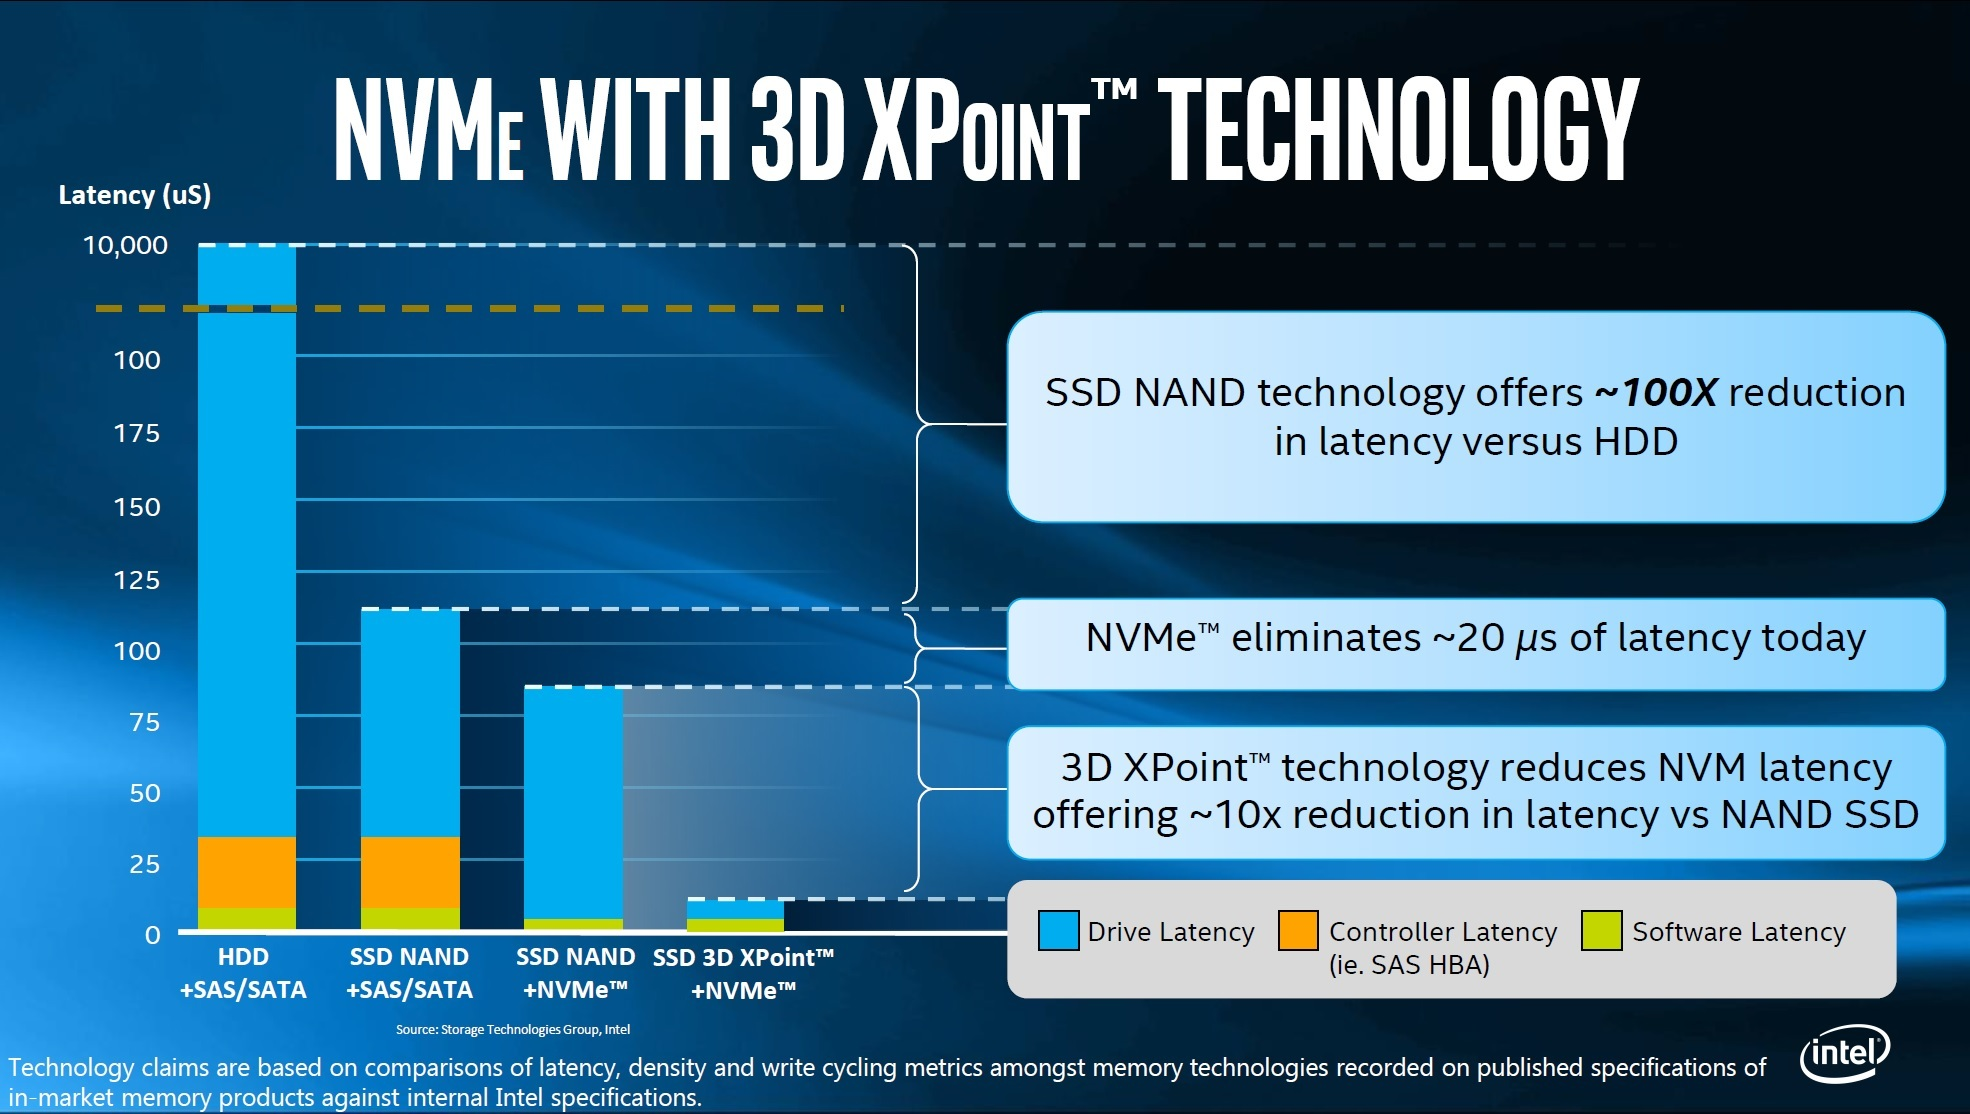
\includegraphics{images/storage_intel.jpg}
      \caption{Storage types comparison}
      \label{fig:storage_intel}
      NVMe basically removes the orange part of the figure, which is the latency introduced by the controller, since it is a \textit{controller-less protocol} and allows to access the storage directly from the PCIe bus.
   \end{figure}
\end{paracol}


\framedt{
   \textit{Why would a 15TB disk be better than a 27TB disk?}\\
   }{
      \note{Assume the same performance, and the same price.}
      It would be preferrable because \ul{it would take less time to extract all the data from the disk}\footnotemark[1], since it is smaller.
      
      However, large capacity drives are used for \textit{cold storage}, where the data is not accessed frequently, speed is not a priority, and even if the data is accessed, only a portion of the disk is needed at a time; in case of failure and thus needing to retrieve an entire backup, the time taken to retrieve the data is not a priority, since this ---hopefully--- happens only ``once''.
      }
      
\footnotetext[1]{i.e. taking advantage of the space provided}
\section{SSDs - QLC and TLC}
SSDs were invented by Toshiba back in 1980, but they were not popular for almost 30 years, until they eventually became cost-effective. Sometimes extra size in SSDs is used for redundancy, to increase the lifespan of the disk e.g. on a 30TB disk, only 10TB are used, the rest is used for redundancy, extending x3 the lifespan of the disk.

\note{DWPD stands for \textit{Drive Writes Per Day}, and is a measure of how many times the disk can be written to in a day. It can be calculated as $\frac{TBW}{365\times\textit{Years of Warranty}\times\textit{capacity}}$}.

TLC stands for \textit{Triple Level Cell}, and QLC stands for \textit{Quad Level Cell}. The difference between the two is the number of bits stored in each cell. The more bits stored in each cell, the cheaper the disk is, but the slower it is. The more bits stored in each cell, the more difficult it is to read and write the data, and the more difficult it is to keep the data stored in the cell.

Generally QLC disks are used for cold storage, while TLC disks are used for hot storage.
TLC in general is more reliable than QLC, has a longer lifespan and better performance, however they cost more.

\section{Storage Concepts}
\subsection{Tiering - Memory Hierarchy}

\begin{figure}[htbp]
   \centering
   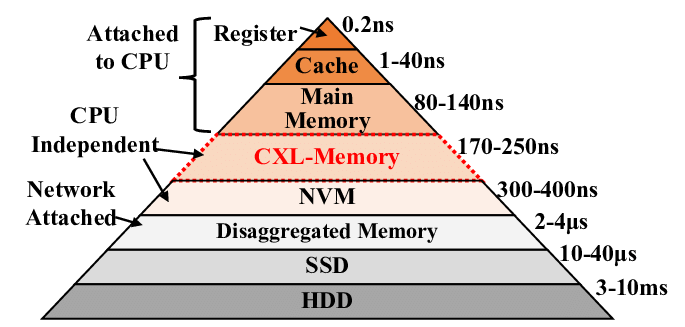
\includegraphics{images/tiering_memory.png}
   \caption{Memory tiering hierarchy}
   Ram could actually be split in \texttt{RAM} and \texttt{nvRAM} (Non-volatile \texttt{RAM}, uses \texttt{nvDIMM}), which is used to store the data in case of a power failure.
   Sometimes, \textit{tape} is included in the hierarchy, because it is used for long-term storage, and it is very cheap.
   \label{fig:tiering_memory}
\end{figure}

Tiering consists in categorizing the data in different categories, and storing the data in different types of storage, depending on the category. The data that is accessed more frequently is stored in the fastest storage, while the data that is accessed less frequently is stored in the slowest storage. This allows to increase the performance, and to reduce the cost. 

\subsection{IO operations, are they all the same?}
\textbf{IOPS} (Input/output operations per second) is an input/output
performance metric used to characterize computer storage devices; it is associated with an access pattern: \textit{random} or \textit{sequential}.

\subsubsection{Random vs Sequential access}

Before explaining the distinction, is important to remember the concept of \textit{queues}: for each thread, the OS can implement a series of queues to solve asynchronously the I/O requests. Using multiple queue can make performances better, since having
the OS to manage parallel requests will increase throughput.
If the queries are latency sensible, not using a queue is better, since
it allows a single query to have ``max'' priority.

\textit{Random access files} are advantageous in scenarios where frequent direct access or modification of specific records is required, while \textit{sequential access files} are advantageous in scenarios where frequent reads of the full files are required. The disk behaves differntly in case of access of those files.

To have a full picture of random vs sequential access, check this site: \url{https://www.prepbytes.com/blog/general/difference-between-sequential-and-random-access-file/} 

\newpage
\subsubsection{Cisternino's demo}
Prof. Cisternino showed a demo in class, where he used a tool to measure the IOPS of a disk.
\begin{figure}[htbp]
   \centering
   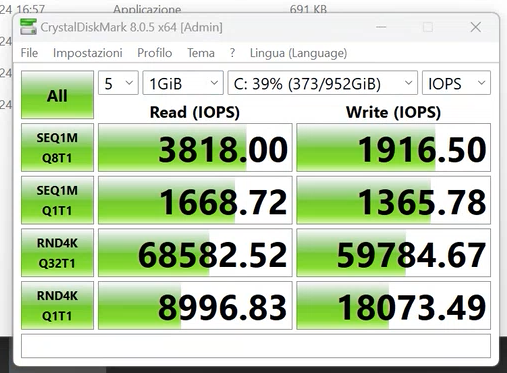
\includegraphics{images/iops.png}
   \caption{IOPS demo; respetively}
   \label{fig:iops}
\end{figure}

\ul{Recall that IOPS by itself is meaningless!} It is a number that must qualified and put in relationship with something else.

\subsection{Latency and Storage Aggregation}
A mechanical hard drive introduces 2.71\% of latency when reading, for instance, 40MB of data.  Optane can perform 416 accesses in the same time needed by a mechanical hard drive to perform 1 access. It looks like the latency in this latter case is neglegtible. Someone may be tempted to reduce the size of read/write operations and perform multiple smaller ones, since ``it's free''. 

Latency in general is due to:
\begin{itemize}
   \item \textbf{Software}\\
   $\mu s$ order which cannot be removed
   \item \textbf{Controller}\\
   Taken down to $20\mu s$ with NVMe (even $2.8\mu s$ according to Copilot)
   \item \textbf{HDD latency}\\
   This was drastically reduced with SSDs and got even less with 3D NAND.
\end{itemize}
Latency may be solved by \textbf{storage aggregation}, which consists in aggregating multiple storage devices into a single logical unit, in order to increase the performance and reliability.
Even if the data is split in multiple disks, the whole system is ``pictured'' as a single huge drive\footnote{\textit{``Cloud resource pooling''} rings a bell?}, making a huge difference in terms of latency, since multiple \texttt{read/write} requests may be sent in parallel to multiple disks.

\newpage
\subsection{Storage Fabric - Fibre Channel}
\textbf{Fibre Channel} is the fabric dedicated to storage; the link coming from the storage ends up in the \textit{HBA} (Host Bus Adapter) in the server.
\begin{paracol}{2}

   \colfill
   The idea is to have an interface which announces itself as drive and that manages the remote storage through Fibre Channel.
   Fibre Channel typically runs on optical fiber cables, but may also run on Ethernet cables (FCoE).

   In Fig. \ref{fig:fibrechannel} is depicted the ideal architecture for Fibre Channel, where the storage is connected to the network through a switch, and the servers have a dedicated HBA to connect to the storage.
   \colfill
   
   \switchcolumn
   \begin{figure}[htbp]
      \centering
      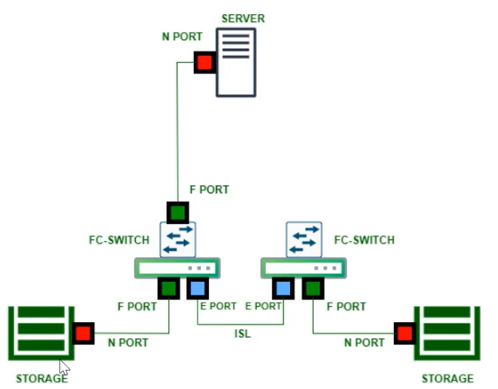
\includegraphics{images/fibrechannel.png}
      \caption{Fibre Channel desired architecture}
      \label{fig:fibrechannel}
   \end{figure}
   
\end{paracol}

\begin{figure}[htbp]
   \centering
   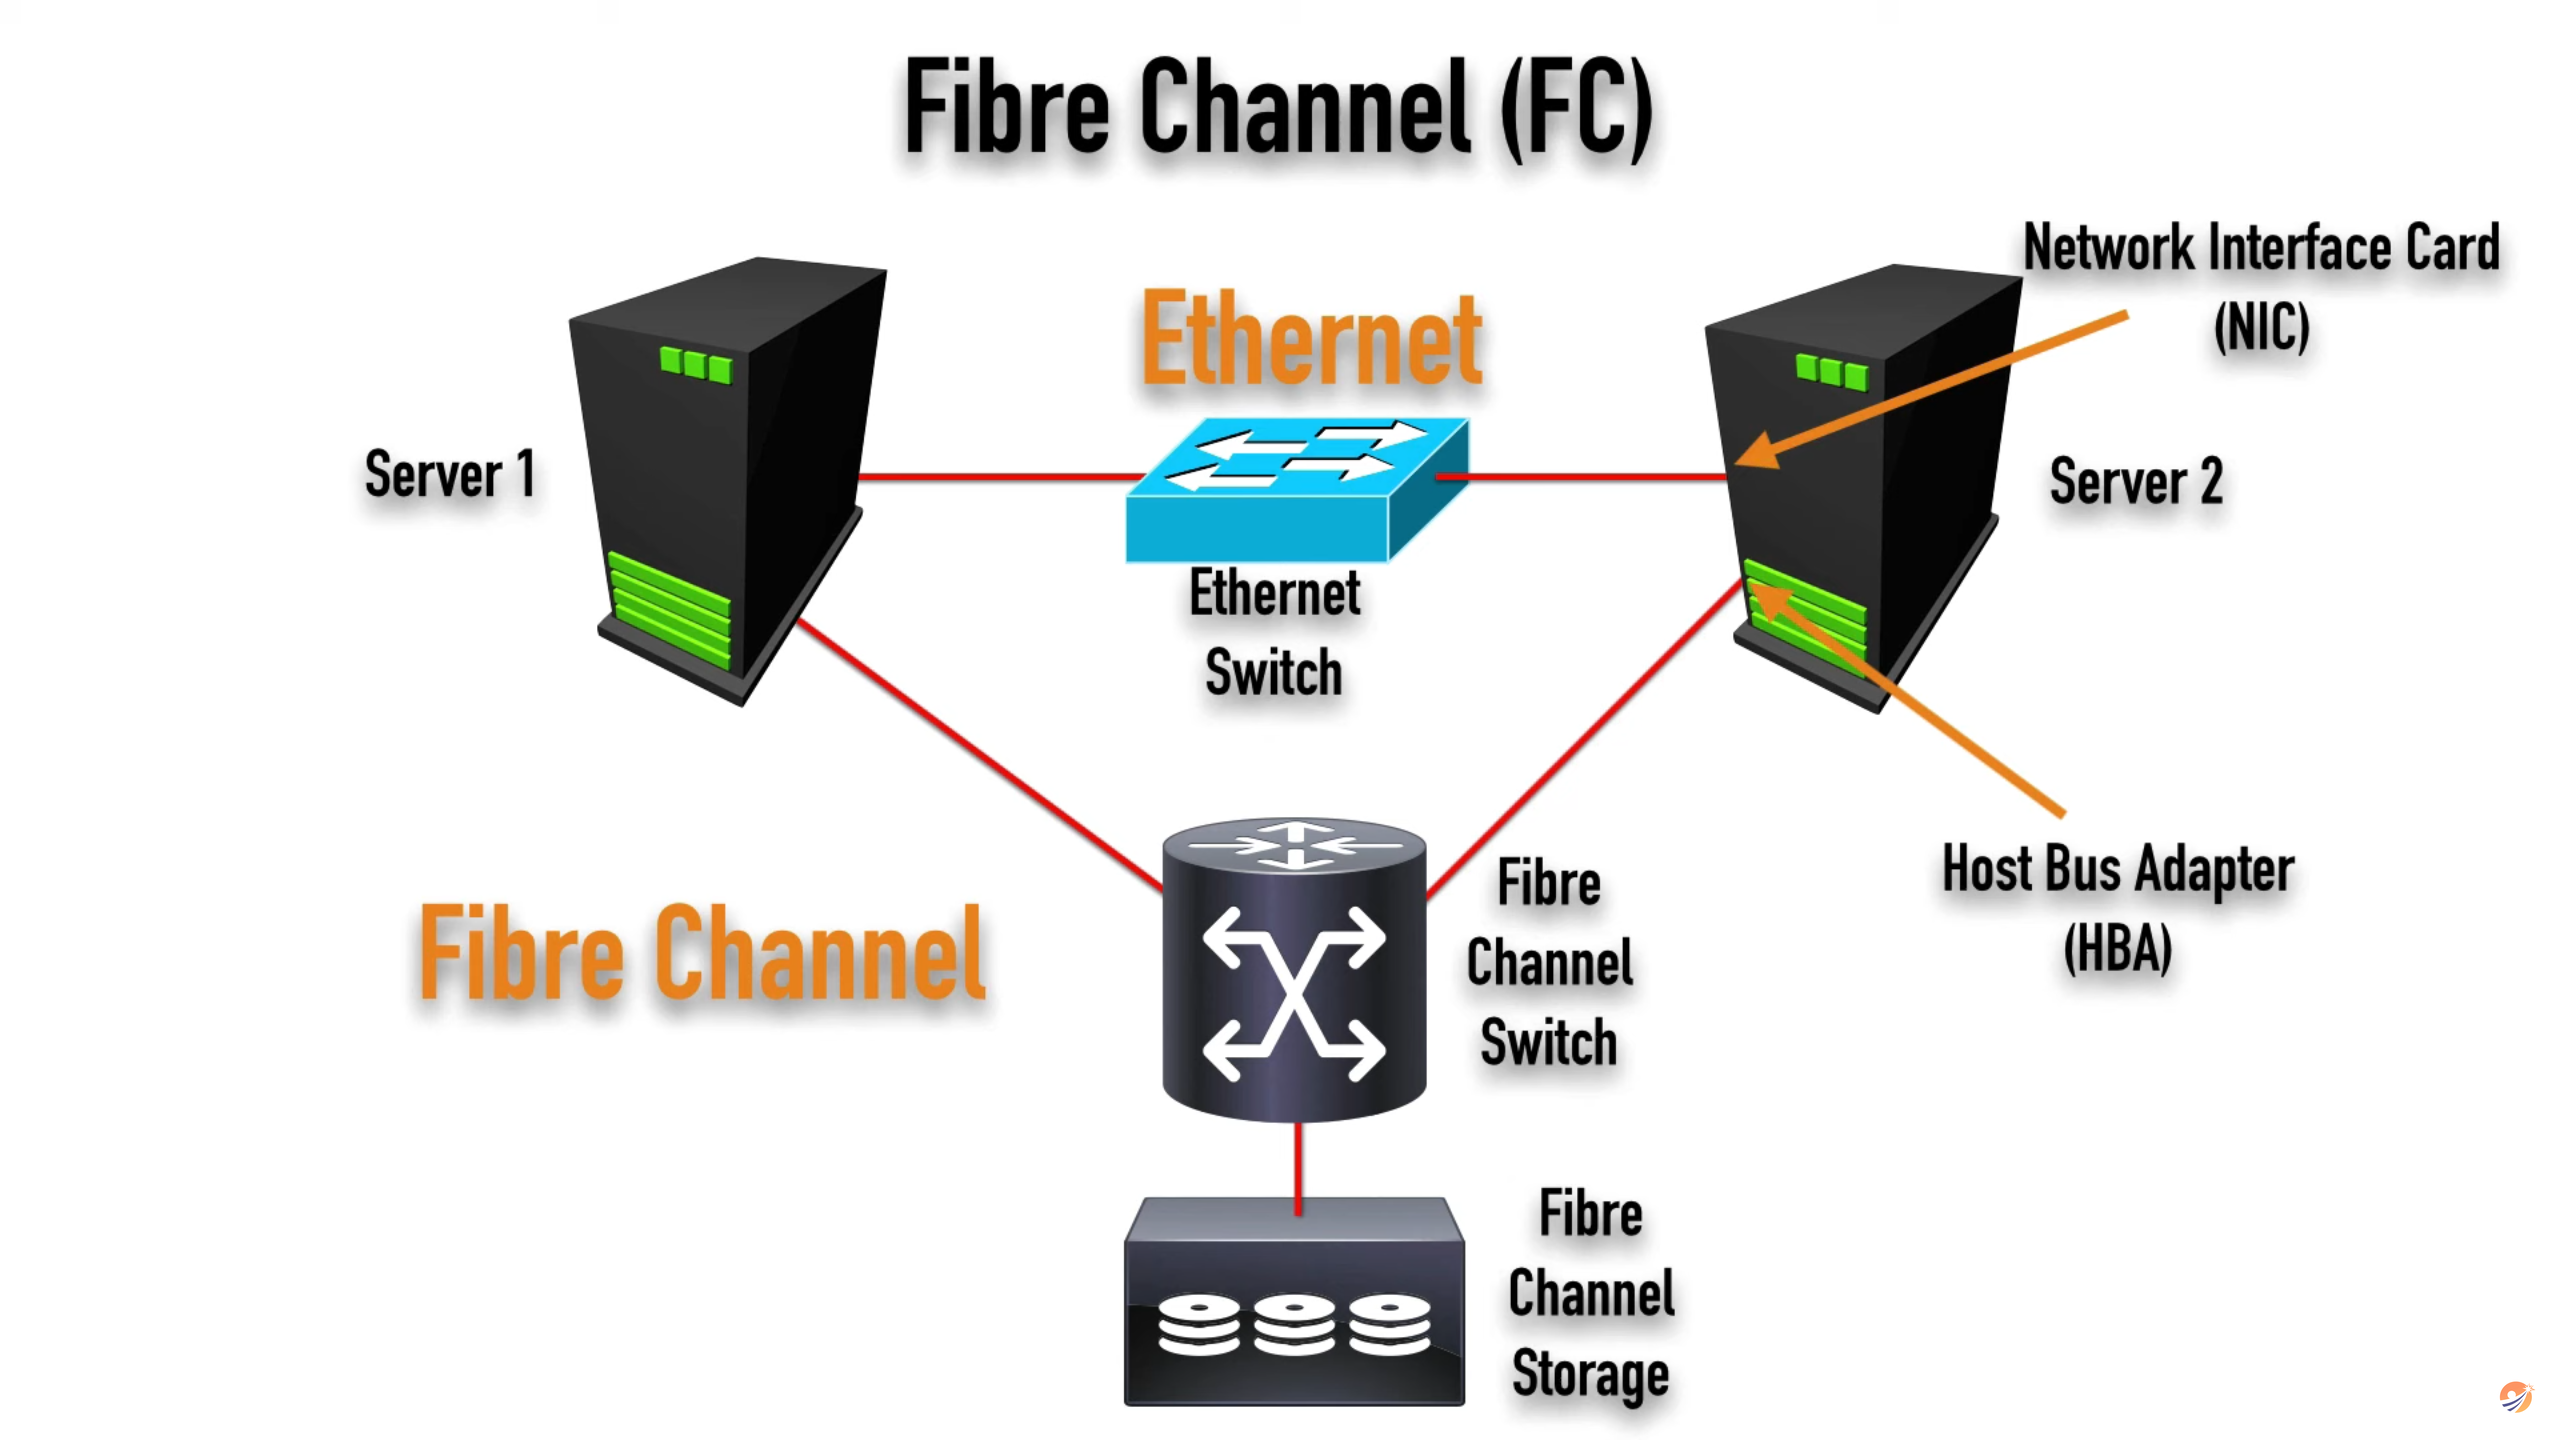
\includegraphics[width=0.32\columnwidth]{images/storage_fabric1.png}
   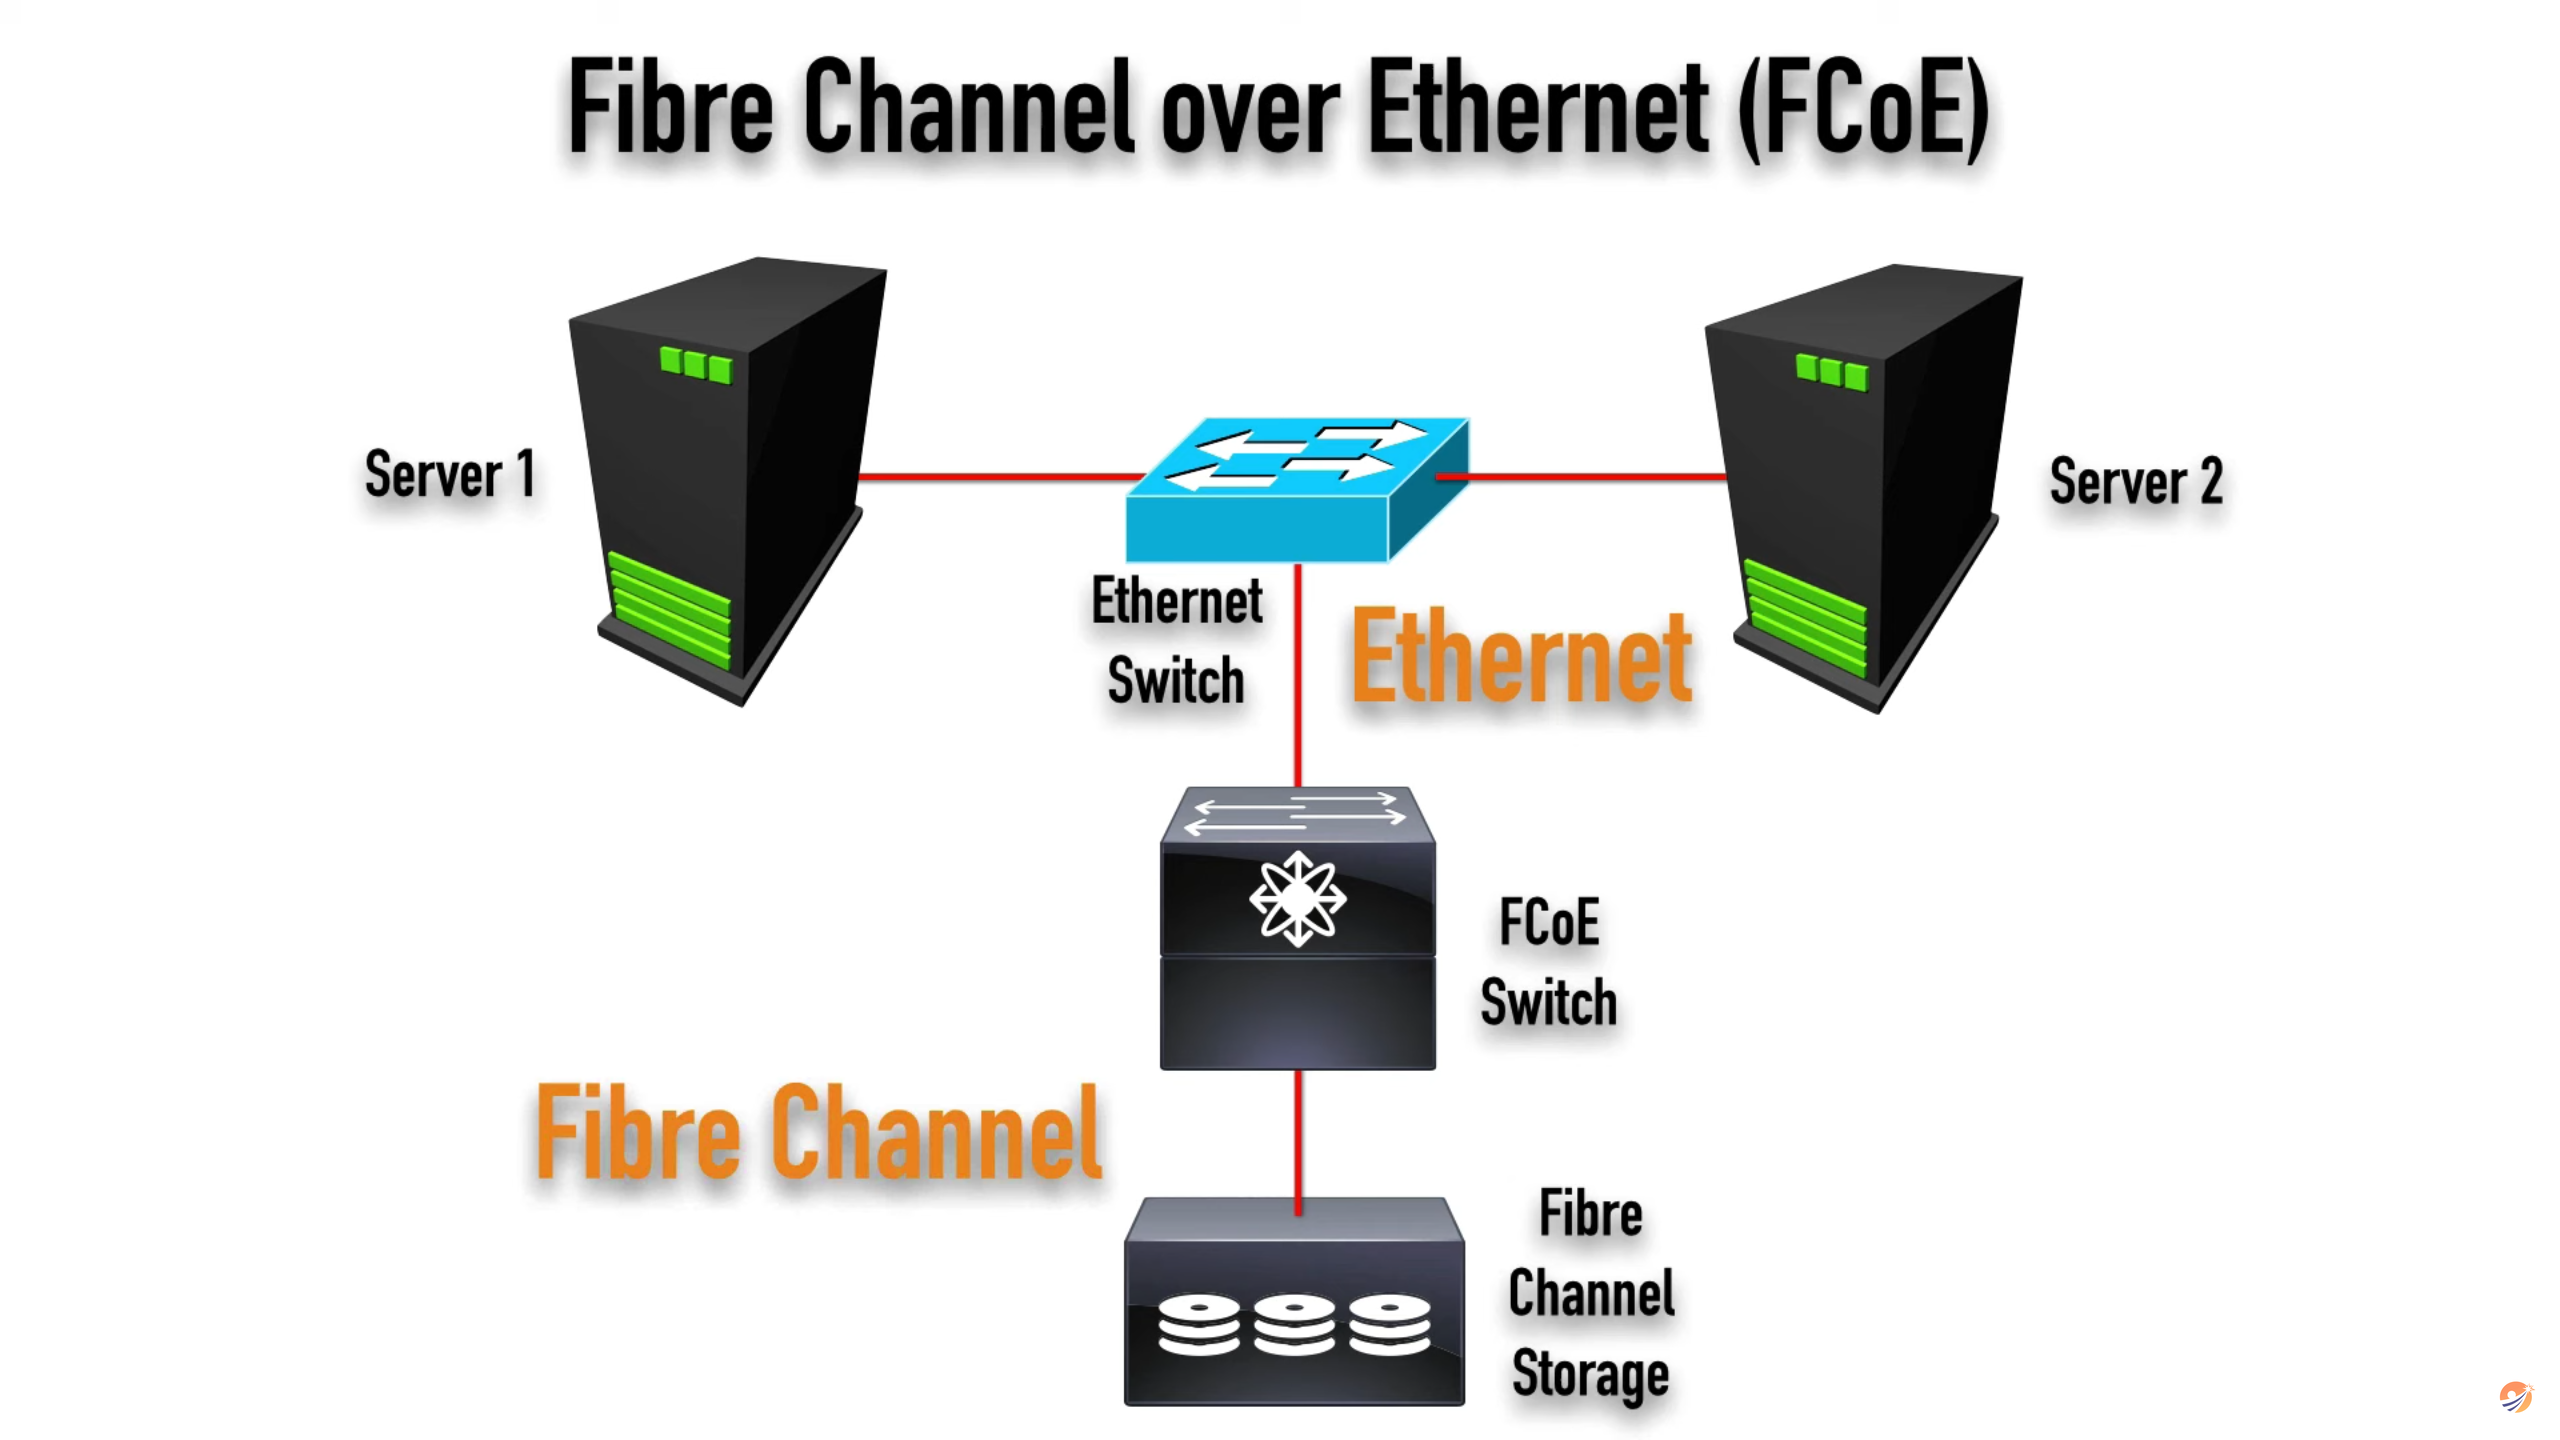
\includegraphics[width=0.32\columnwidth]{images/storage_fabric2.png}
   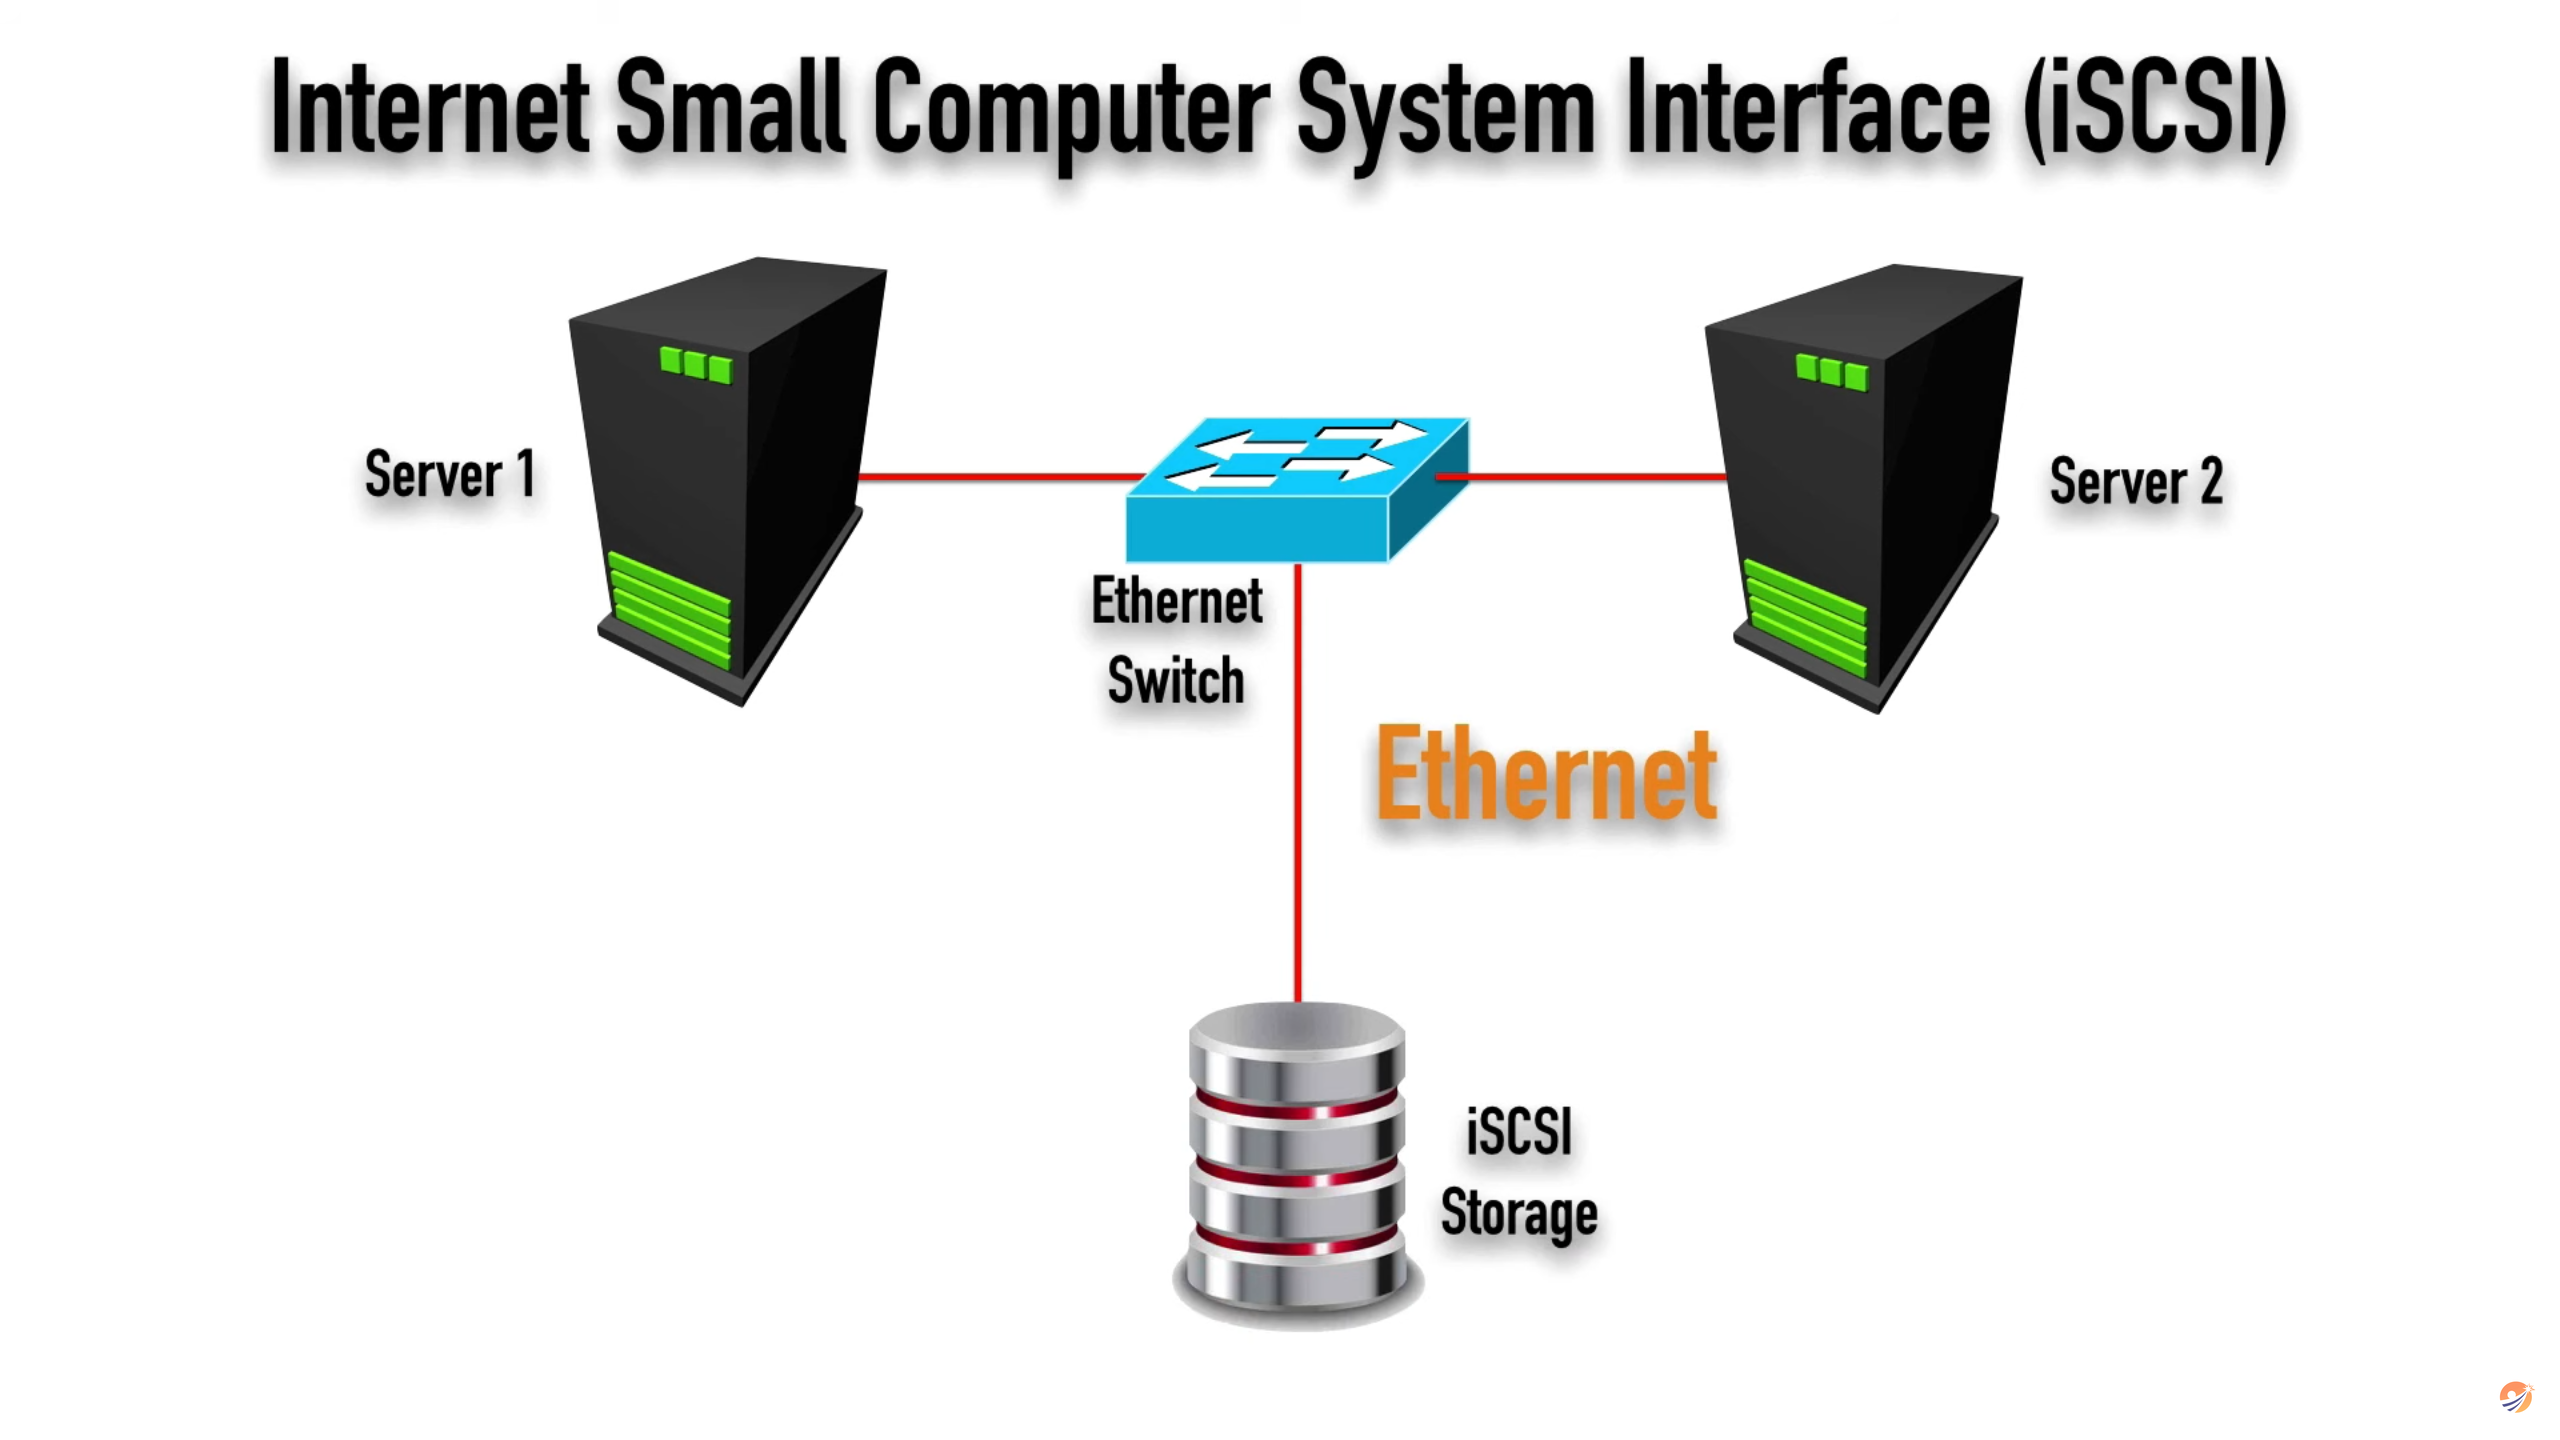
\includegraphics[width=0.32\columnwidth]{images/storage_fabric3.png}
   \caption{These are three possible configurations for the storage fabric, the first being the most performant, and the third being the cheapest.
   Note that in the second picture the first link is Ethernet and the second is Fibre Channel.}
   \label{fig:storage_fabric}
\end{figure}
Note that the image may me misleading, since there may be multiple FC switches (as partially depicted in Fig. \ref{fig:fibrechannel}) and multiple storage racks.
   
\subsection{Bus, controller and some numbers}
A bus is a component to whom multiple devices may be attached. It has a clock and some lanes, 16 in the case of PCI, each one providing almost 1GB bandwidth, summing up to $\sim 15GB$: 4 drives are enough to saturate a full PCI bus, or a 100Gbit link ($12.5GB/s$).;
in fact an NVMe SSD has a bandwidth of 3.5GB/s, hence $3.5\times 4 = 14GB/s \simeq 15GB/s$.\\
NVMe is often used in the lower memory tier of the RAM: its speed is only one order of magnitude less than RAM, but can provide high capacity without any problem.
It may represent a valid super-fast cache level for the RAM and hence started being associated in one single level to implement a big RAM tier, in a totally transparent way for the system.

Since the software latency in disk IOs is 5 microseconds more or less,
TCP/IP software introduces also a latency of 70-80 microseconds, the disk is
no more a problem. Indeed, the problem is now the network, not only for the
latency, but also for the bandwidth: as stated before 4 NVMe totally saturate a 100 Gbps
link.

\section{Redundancy and backup}
\subsection{Checkpoints}
It's unpractical for a system to go down after 5 months. For this reason it is necessary to have \ul{\textit{checkpoints}, which are points in time where the system can be restored to.} The system can be restored to the last checkpoint, and the data that was written after the checkpoint can be re-applied. This is similar to what happens to applications on smartphones are closed and then re-opened, the application is restored to the last checkpoint.

\subsection{RAID}
\textbf{RAID} stands for \textit{Redundant Array of Independent Disks}. It is a technology that allows to combine multiple disks into a single logical unit, in order to increase the performance, the reliability, or both. There are different levels of RAID, each with different characteristics.

Historically \textit{Redundant Array of Inexpensive Disks}, because it was more common for disks to eventually fail, so RAID was the only countermeasure to this. Today, disks are more reliable, so RAID is used more for performance reasons.

In RAID, \textbf{XOR} is used to calculate the parity of the data. The parity is used to recover the data in case of a disk failure. The parity is calculated by XORing the data of the disks. The parity is stored on a separate disk, called the parity disk. The parity disk is used to recover the data in case of a disk failure.


\section{Network sharing architectures}
Before going into the details of the architectures, it is important to understand the difference between \textbf{protocols} and \textbf{architectures}.\\
\textbf{SMB/CIFS} is a protocol that allows to share files over the network. It is used by Windows, but it is also supported by Linux and MacOS. NFS is a protocol that allows to share files over the network, it is used by Linux and MacOS, but it is also supported by Windows.\\
NFS is faster than SMB, but it is also less secure. SMB is slower than NFS, but it is also more secure.\\
These however are protocols for file sharing, not properly ``architectures''.

\framedt{Capacity and system architecture}{
   When we talk about \textbf{capacity}, there are two measures which we can refer to:
   \begin{enumerate}
      \item \textit{Scale-\textbf{up}}:
      adding more disks to the same server
      \item \textit{Scale-\textbf{out}}:
      adding more servers to the same network
   \end{enumerate}
}

\subsection{File based - NAS}
\textbf{NAS} are devices that are connected to the network, and that are used to store files, providing aggregated capacity. They are used to store files that are accessed by multiple users, and that need to be accessed from multiple devices.
NAS systems have integrated HW and SW component, including CPU, memory, NICs, optimized OS for file serving, file sharing protocols and so on.\\
Typically they exploit SMB/CIFS or NFS protocols, or AFP over optical fiber, and represent a good solution for \textit{document management}.

\subsection{Block based - SAN}
\textbf{SAN} stands for \textit{Storage Area Network}, which enables the creation and assignment (i.e. access and share) of storage volumes to compute systems.\\
The compute OS (or hypervisor) discovers these storage volumes as local drives.
The servers have different NICs (HBA) connected (usually through
fibre channels) to those blocks, which are aggregated volumes.\\
SAN also enables performance optimization of the storage by performing
deduplication (delete sequence of blocks that are equivalent).

\note{HBA stands for \textit{Host Bus Adapter}, and is a device that allows to connect a computer to a storage device. It is used to connect a computer to a storage device, and to allow the computer to access the storage device.}

SAN are a network separate from the LAN, so not affected by its traffic.\\
They usually exploit Fibre Channel or iSCSI (which is not as fast) protocols.

SAN was, before SSDs, one of the datacenter pillars.
Its architecture included a ``head'', an advanced Fibre Channel switch, to which drives were attached, and the head was connected to the network. The head was used to manage the drives, and to allow the servers to access the drives.\\
When SSDs became popular, the head became a bottleneck, because it was not able to keep up with the speed of the SSDs(Recall that 4 SSDs are enough to saturate a 10Gbit link, See Sec. \ref{sec:bandwidth_storage}). 
For this reason, the head may be removed, with the drives connected directly to the servers. This is called \textbf{DAS}, typically uses SCSI protocol, but is not as scalable as SAN.

However with groups of mechanical drives, ---if the data is splitted in a smart way--- it's possible to be faster of a single SSD, since the request will be forwarded in parallel to different drives.

\subsubsection{Protocols}
SANs are classified based on protocols and fabric they support. Some possible configurations can be found in Fig. \ref{fig:storage_fabric} 
Common SAN deployments types are Fibre Channel SAN (FC SAN), Internet Protocol SAN (IP SAN), and Fibre Channel over Ethernet SAN (FCoE SAN), ATA over Ethernet (AoE) and HyperSCSI ().
It can be implemented as some controllers attached to some JBoDS (Just a Bunch of Disks).

\note{While NAS provides both storage and a file system, SAN provides only block-based storage and leaves file system concerns on the “client” side.
However, note that a NAS \textit{can} be part of a SAN network.}


\subsubsection{Pools and LUNs}

\textbf{Storage pools} are used to combine multiple storage devices into a single logical unit, in order to increase performance and reliability. 

The SAN is divided in different Logical Unit Numbers (\textbf{LUN}s), which abstract identity and internal functions of storage devices, and appear as phyisical storage to the compute system.\\
\textbf{Storage LUNs} define a storage partition and are used to assign storage ---a portion of the pool--- to a server, and to allow the server to access the storage, using ACLs.
\nl

In the following section, some LUNs features are listed
\begin{itemize}
   \item 
   Storage \textbf{capacity} of a LUN can be dynamically expanded or reduced
   by means \textbf{virtual storage provisioning}, i.e. present a LUN as if it has more capacity than it actually has, to avoid fragmentatation and then expand it when it is needed.
   \note{e.g. if you assign a 1TB LUN to a server, and then you need to expand the LUN due to lack of space, if you have space next to the already assigned TB you can avoid fragmentation. Besides, if you can put data in only 1TB instead of 2TB (even if you present the volume as if it had 2TB), internal fragmentation may happen only inside that TB, and later on you can expand the volume up to the reserved 2TB.}
   Besides, \ul{available space may \textit{decrease} over time}, mostly due to snapshots (discussed later on).
   \item LUNs may perform \textbf{deduplication} (delete sequence of blocks that are equivalent/redundant, and exploiting indexes to retrieve duplicated data) to optimize storage performance. It is very useful in document-rich file systems, since people tend to copy a document multiple times.
   \item LUNs may perform \textbf{compression} to reduce the size of the data, and to increase the performance. It may be lossy or lossless.  Its major downside is that it is computationally expensive, since the data must decompressed before using it.
   On the other hand, allows to spare bandwidth by sending compressed data, which we know to be critical.\\
   \textit{Searching} in compressed data is not trivial, but there are tools to do it, such as the \href{https://en.wikipedia.org/wiki/FM-index}{\texttt{FM-index}}.
   \item LUNs may create \textbf{snapshots}, \textit{``point-in-time''} copy of current data state, to save the differences between the current state of the data and the previous state of the data. This allows to recover the overwritten data in case of a failure, but it also takes up space.\\
   Snapshots older than a week are usually deleted, since they are not needed anymore.
   
\end{itemize}

\subsubsection{Provisioning and Capacities}
LUNs may be created from\ns
\begin{itemize}
   \item A \ul{RAID set} (traditional approach); suited for application that require predictable performance
   \item A \ul{storage pool} (modern approach); suited for application that require flexibility and scalability, and that tolerate performance variations.
\end{itemize}

Both of these approaches have different capacities:\ns
\begin{itemize}
   \item Row capacity: the total capacity of the LUN, limited by the physical capacity of the storage devices
   \item Usable capacity: the capacity that is available to the server, limited by data structures needed to allocate the file system.
   \item Provisioned capacity: the capacity that you present to the server. May be more than the usable capacity, obtaining overprovisioning. 
\end{itemize}

\subsection{Object based - S3}
\textbf{S3} stands for \textit{Simple Storage Service}, and is a service that is used to store file data in the form of objects based on the content and other attributes of the data rather than the name and location of the file.
The additional metadata (size, date, ownership\dots) or attributes (retention, access pattern\dots) enable optimized search, retention and deletion of objects.\\
A flat, non-hierarchical address space to store data provides the flexibility to \textit{scale massively}.\\
\ul{S3 is leveraged to provide Storage as Service.}

\subsection{Big Data - HDFS}
\textbf{HDFS} stands for \textit{Hadoop Distributed File System}, and is a distributed file system that is used to store large amounts of data across multiple servers.
A \texttt{map/reduce} algorithm is applied on the data, and then results are collected and summarized.\\
It exploits good forms of parallelism to run efficiently the algorithm

\subsection{Unified - Unified Storage}
\textbf{Unified Storage} or multi-protocol storage has emerged as solution that consolidates block, file and object storage into a single storage platform. It supports multiple protocols, such as NFS, SMB, iSCSI, FC, REST and SOAP.

\framedt{iSCSI and its death}{
   SCSI (Small Computer System Interface) was invented in 1979 for chaining drives
   through a bus (used for e.g. in fibre channels). The controller was so smart
   to allow the the drive to share the flat cable as a bus.\\
   Over the time some variants were invented, but the basic idea is the same.
   One example is iSCSI: \textit{Internet Small Computer Systems Interface}, an IP-based storage networking standard for linking data storage facilities.
   It provides block-level access to storage devices by carrying SCSI commands over a TCP/IP network. The protocol died when SSD were introduced, since the latency was too high when communicating over the network.

   The key idea behind SCSI was for \ul{mutiple drives to share the same physical flat cable}.\\
   It had been ``deprecated'' in favor of \texttt{NVMe}, but it is still used today, because it is very reliable.
}
\subsection{Synchronization Software and its Price}
The ``storage guy'' must ensure that there is no condition under which can happen data loss, because it is never an option. It is also important to have powerful \textbf{synchronization algorithms}, which must allow data to be copied and synchronized in multiple locations without disrupting performance and handling concurrency;
such software is typically \textit{costful}.

It is difficult nowdays to establish what is the ``right'' price for software. The shift from highly specialized and costful hardware to general hardware-plus-software, gave the software, which still is a non-physical entity, increasingly more value, perhaps even too much.


\section{Hyperconverged Infrastructure}
SAN started to create a sensible bottleneck, so designers started to ``move drives towards the servers''.
\textbf{DAS} stands for \textit{Direct Attached Storage}, and is a technology that allows to connect multiple storage devices to a single server, in order to increase the performance, the reliability, or both.
The limitations is that you can only attach up to 2 or 3 drives to a server.

An idea came out to use the servers' internal drive to build a Storage Area Network, and this is called \textbf{VSAN}.

\subsection{HCI solutions}
\textbf{HCI} stands for \textit{Hyperconverged Infrastructure}, and is a technology that allows to combine multiple servers into a single logical unit, in order to increase the performance, the reliability, or both. 
The idea was born to allow a scale-out architecture, where you can add more servers to the network.

\begin{center}
   \ul{\textit{``Adding servers adds capacity''}}
\end{center}

The \textbf{Hypervisor} is the software that allows to run multiple virtual machines on a single server. There should be some locality between the VM and the storage, because the VM should be able to access the storage quickly.\\
The \textit{controller VM} (one per host) implements the storage abstraction and the logical moving of data.
\texttt{read} operations are always performed locally on local drives; \texttt{write} operations instead sometimes require to retrieve a remote piece of data.
A copy on the local server storage is kept, but the server needs to wait for the acknowledgment of the remote server in order to keep updated replicas of written data in other nodes.

As mentioned in the section dedicated to HCI and networking Sec. \ref{sec:HCI_network}, new server are automatically added to the network seamlessly integrating with the pre-existing HCI cluster.
The same applies to the storage, which is automatically added to the pool, and local replicas of data are built.

\subsubsection{VM Live Migration}
Live Migration of VMs is a technique that allows to move a VM from one server to another server, without interrupting the service. 
When it happens over SAN there's no need to copy storage to the new server, since the storage is shared and accessed through the network.
The case of HCI is similar since the storage is mostly shared, but there are also the above mentioned local copies of data, which may need to be updated. 

\subsection*{Riak and Acropolis}
Riak is a distributed database that is used to store data in multiple locations. 
The same applies to Acropolis, which is a distributed storage system.

Recently it has been recognized that \ul{using general purpose hardware is no longer a feasible option.}

\section{SDS - Software Defined Storage}
\textbf{SDS} \textit{Software Defined Storage} refers to software for policy-based provisioning and management of data storage independently from the underlying hardware.
Such software is more costful than the hardware it is running on, since it also optizimes the drives, not simply managing them.\\
SDS exploits object-based storage architecture and DHTs to provide storage services.
\chapter{Attacks}
% \section*{3 - Ottobre}
\section{Attacks and Vulnerabilities}
Following the discovery of a vulnerability $v$ there's an analysis to evaluate which attacks are enabled by $v$.
\textbf{Attacks} can be described as a set of attributes:
\begin{enumerate}
    \item Precondition
    \item Postcondition
    \item Success Probability
    \item Know how, abilities, tools required
    \item Noise = Probability of being discovered
    \item Automated/Potentially automatable/manual
    \item Local/Remote
    \item Actions to implement attack\footnote{See following Section on attack taxonomy}
\end{enumerate}
Even though some attack evaluation proposals map to each attribute a number and combine them into a value,
such evaluations do not consider that \textbf{risk} resides in \textit{intrusions}, not individual attacks, because they have a considerable impact on the system, and keep in mind that are composed by:
\begin{itemize}
    \item Exploration and information collection
    \item Persistence
    \item Attack \textit{chain} for privilege escalation
\end{itemize}

\section{Attack Classification}
\label{sec:attack_taxonomy}
The actions need to implement an attack may be used to define a \textbf{taxonomy} of attacks:
\begin{enumerate}
    \item buffer/stack/heap overflow
    \item \textit{sniffing} $\rightarrow$ Illegal access to info in travel
    \item \textit{replay attack} $\rightarrow$ Repeated exchange of legal messages 
    \item \textit{Interface attack} $\rightarrow$ Illegal order in the invocation of API functions
    \item \textit{Man-in-the-middle} $\rightarrow$ Interception and manipulation of info in travel
    \item Diversion of an information flow
    \item \textit{Race-condition} $\rightarrow$ Time-to-use time-to-check
    \item \textit{Cross site scripting} $\rightarrow$  XSS
    \item SQL injection
    \item \textit{Bell-Lapadula policy} $\rightarrow$ Covert channel 
    \item Masquerading as
    \begin{itemize}
        \item user
        \item machine (\textit{IP/DNS spoofing, Cache poisoning}
        \item connection (\textit{connection stealing/insertion})
    \end{itemize}
\end{enumerate}

\section{Examining attacks}
\subsection*{Replay attack}
Suppose a user asks the bank to transfer some money to $Y$ account with an $M$ message.
$Y$ may sniff and record $M$, and before the secure channel $S$ gets deleted, $Y$ sends $M$ several times.\\
Note that the attack may work even if encryption is used.

\subsection*{Man-in-the-middle}
If $A$ and $B$ communicate, $E$ may pose itself in the middle, acting as if it were $B$ to $A$ and $A$ to $B$.
Such attack is possible when no authentication is required.

\subsection*{XSS}
A website allows users to upload contents to be later (possibly) downloaded by users.
Thus a malicious user may upload hidden scripts to damage or steal information from the user who download their content.
To avoid this the website must check the content uploaded by users.\\
A well known attack of this type targeted BBC.

\subsection*{SQL Injection}
An input may insert a malicious query (i.e. \lstinline[language=SQL]{DROP TABLE USERS}) in a credentials field.
The best way to avoid this is to whitelist using RegEx.

\subsection*{Cryptography attacks}
These are a category on their own, there are many types, with different variations and features.

\subsection*{Side-channel attacks}
Any attack that measures some physical value to discover an encryption key.
Currently it is popular due to the capabilities of machine learning in exploiting large number of pairs to deduce a function.\\
Such measures may be:
\begin{itemize}
    \item Electromagnetic emissions
    \item Energy consumption
    \item Execution time to discover inner status
    \item Execetion time to discover cache usage and prediction mechanisms.
\end{itemize}

\subsection*{Virtual Machines \& Blue Pill}
Cyber system may be composed of many virtual machines onion-like organized.
Thus, attacking a low-level VM may grant access rights to higher ones.\\
Besides, an attacker may insert a new VM in the hierarchy:
this is called \textit{Blue Pill} attack, it's hard to discover and has a high impact.
A new VM may return to higher VMs fake information on the status of the underlying machines and/or send malicious commands to the underlying machines.\\
\texttt{Stuxnet} was a malware which used to send commands to uranium enrichment centrifuges to destroy them, and meanwhile told the operator that everything was going well.  

\chapter{Cloud computing}
\section*{19 - Ottobre}
Powerful hardware and high-speed networking have made room for the development of cloud computing.
\textbf{Cloud computing} allows virtual resources accessible \textbf{on demand},
and provides many advantages against the standard old-style scaling methods i.e. buying resources.
\begin{itemize}
   \item \textit{Scalability}
   \item \textit{Elasticity}
   \item \textit{Resilience}
   \item \textit{Cost}
\end{itemize}

\section{Virtualization and Containers}
\begin{paracol}{2}
   Virtual machines on a single physical machine are managed by hypervisor
   \begin{table}[!htbp]
      \centering
      \begin{tabular}{|cc|}
         \hline
         App A & App B\\
         bins/libs & bins/libs\\
         Guest OS & Guest OS\\
         \midrule
         \multicolumn{2}{|c|}{\textbf{Hypervisor}}\\
         \hline
         \multicolumn{2}{|c|}{Host OS}\\
         \hline
         \multicolumn{2}{|c|}{Hardware}\\
         \hline
      \end{tabular}
   
   \end{table}

   \vspace{\fill}
   \switchcolumn

   Containers instead exclude one layer of abstraction, saving up a lot of resources
   \vspace{\fill}
   \begin{table}[!htbp]
      \centering
      \begin{tabular}{|cc|}
         \hline
         App A & App B\\
         bins/libs & bins/libs\\
         \midrule
         \multicolumn{2}{|c|}{\textbf{Container Manager}}\\
         \hline
         \multicolumn{2}{|c|}{Host OS}\\
         \hline
         \multicolumn{2}{|c|}{Hardware}\\
         \hline
      \end{tabular}
   \end{table}

   \vspace{\fill}
\end{paracol}

\section{Docker}
Docker exploits container-based virtualization to run multiple isolated guest instances on the same SO.
Software is packaged into \textbf{images} which are read-only templates to instantiate and run containers.
External \textbf{volumes} can be mounted to ensure data persistance when used by multiple containers or by the host machine.

It is possible to \textbf{stack} multiple docker \textit{images},
and if desired create a new image as a result of stacking other ones.
\chapter{Containers}
\label{chap:containers}

\ul{A VM is better than a process because it provides \textbf{isolation}}:
a typical problem in cybersec is that if an attacker cracks a process, he may access the whole system;
with a VM, the attacker can only access the VM, not the host.
However, a VM introduces overhead due both to the hypervisor and to the OS (cache, kernel, storage management\dots).

\note{The idea is to tell a process that a process that its root is a subdirectory of the host's root, resulting in a strong isolation.}

\textbf{Docker} provides a \textit{differential filesystem}, which is a filesystem that is a diff of the host's filesystem, an abstraction where the new ``inner'' file system is based on a given one, where the system will only store the differences between the original file system and the new one.

Docker has become the de facto standard for containers, but there are other solutions like \textbf{LXC} (Linux Containers) and \textbf{rkt}.
A Dockerfile contains the information to build a container.

One of the key differences between a VM and a container is that containers \textbf{do \textit{not} have a virtual switch}.
A container uses the same MAC address of the host.\\
Docker containers are processes, and only see a portion of the host's filesystem.

Inside a Dockerfile you may create temporary containers by exploiting multiple images and lastly build the resulting slimmed image.

\section{Upgrading a system}

Typical procedure when a system needs to be updated: create first a snapshot before updating the containers (especially if there are updates related to the database), then update, run back the containers, check if everything works, and then delete the snapshot. If anything goes wrong, the snapshot will help to roll back.

\section{Docker compose}
Docker compose is a tool to define and run multi-container Docker applications. It uses a YAML file to configure the application's services, networks and volumes. With a single command, you can create and start all the services from your configuration.

Kubernetes is a more advanced tool for container orchestration, way more complex than Docker compose, it allows to manage thousands of containers, providing fundamental scalability features.

\section{Docker security}
An attack is to put the machine under heavy workload and observe from the container the performance to infer what other processes may be. This is called \textbf{side channel attack}.

Google has thousands of VMs and each runs a \textit{container for each query}.
\chapter{Cloud}
Cloud came out as a business model, not as a technlogy.
It was needed to handle peak of requests and to allow scalability, without oversizing Infrastructures.
\note{e.g. Amazon needs to handle way more requests on Christmas than on a normal day.}
So, Cloud was a mean to reduce the cost of the ICT infrastructure.

\textbf{Resource pooling} is the key concept of Cloud. It means that the services are provided to users using a multi-tenant model, with physical and virtual resources being dynamically allocated and deallocated according to the demand.\\
Cloud was needed also to provide rapid elasticity, meaning that capabilities may be elastically provisioned and released, in some cases automatically, to scale rapidly outward and inward commensurate with demand. To the customer it means that the capabilities available for provisioning often appear to be unlimited and can be appropriated in any quantity at any time.

Benefits of Cloud:
\begin{itemize}
   \item \textbf{Business agility}
   \begin{itemize}
      \item Quick resource provisioning
      \item Facilitates innovation
      \item Reduces time to market
   \end{itemize}
   \item \textbf{Reduces IT costs}
   \begin{itemize}
      \item Reduces up-front capital expenditure (CAPEX)
      \item Improves resource utilization
      \item Reduces operational expenditure (OPEX)
   \end{itemize}
   \item \textbf{High availability}
   \begin{itemize}
      \item Ensure resource availability based on customer's requirements
      \note{In RAI, prof. Cisternino experienced people complaining because their servers' CPUs were running at 98\% of their capability, and they wanted to exploit also the remaining 2\%, because ``they paid for it''.}
      \item Enables fault tolerance
      \note{Recall active-active, active-passive, etc. configurations.}
   \end{itemize}
   \item \textbf{Business continuity}
   \item \textbf{Flexible Scaling}
   \item \textbf{Flexibility of Access}
   \item \textbf{Application Dev and Testing}
   \item \textbf{Simplified infrastructure management}
   \item \textbf{Increased collaboration}
   \item \textbf{Masked complexity}
\end{itemize}
Cloud has the magic power of decoupling the software from the hardware.

Disadvantages of Cloud:
\begin{itemize}
   \item Vendor lock-in
   \item Privacy
   \item Your software depends on someone else
   \item Legislation is complicated
   \note{In EU public administration data, must be stored in the EU.}
   \item \dots TODO
\end{itemize}

\section{Cloud Service Models}
\begin{itemize}
   \item \textbf{IaaS} (Infrastructure as a Service)
   \begin{itemize}
      \item Provides virtualized computing resources over the Internet
      \item Examples: Amazon EC2, Google Compute Engine, Microsoft Azure
   \end{itemize}
   \item \textbf{PaaS} (Platform as a Service)
   \begin{itemize}
      \item Provides a platform allowing customers to develop, run, and manage applications without the complexity of building and maintaining the infrastructure
      \item Examples: Google App Engine, Microsoft Azure, Heroku
   \end{itemize}
   \item \textbf{SaaS} (Software as a Service)
   \begin{itemize}
      \item Provides software applications over the Internet
      \item Examples: Google Apps, Microsoft Office 365, Salesforce
   \end{itemize}

\section{Cloud Deployment Models}
\begin{itemize}
   \item \textbf{Public Cloud}
   \begin{itemize}
      \item Owned and operated by third-party cloud service providers
      \item Deliver computing resources over the Internet
      \item Examples: Amazon Web Services (AWS), Microsoft Azure, Google Cloud Platform
   \end{itemize}
   \note{It does \textbf{not} mean that the data is public. It means that the cloud services are accessible to the public.}
   \item \textbf{Private Cloud}
   \begin{itemize}
      \item Operated solely for a single organization
      \item Managed by the organization or a third party
      \item \textit{On-premise} or \textit{off-premise}
   \end{itemize}
   \note{It does \textbf{not} mean that the data is private. It means that the cloud services are accessible only to the organization e.g. \textit{UniPi}.}
   \item \textbf{Hybrid Cloud}
   \begin{itemize}
      \item Composition of two or more clouds (private, community, or public) that remain unique entities but are bound together, and resources may be moved from one cloud to another (with some performance cost obviously) 
      \item By standardized or proprietary technology that enables data and application portability
   \end{itemize}
   \item \textbf{Community Cloud}
   \begin{itemize}
      \item Shared infrastructure for specific community
      \item Managed by organizations or third party
      \item On-premises or off-premises
   \end{itemize}
\chapter{Deception with Honeypots}
A \textbf{honeypot} is a system designed exclusively to be attacked an to \textbf{collect information} about the attacker and its tactics, techniques and procedures;
the other focus of an honeypot is also to possibly slow down an attack to a system by \textbf{diverting} it on itself.

The scaled version of a honeypot, is a \textbf{honeynet},
which is an entire network attached to a real system designed to be targeted instead of the main system.

\subsection{Classification}
\begin{enumerate}
   \item \textbf{Interaction}-based
   \begin{enumerate}
      \item \textit{Low} - e.g. simple port listener
      \item \textit{Medium} - emulation of a network service that analyzes the inputs and returns some replies similar to those the real service would return.
      \begin{itemize}
         \item Simulates just some \textbf{features} of the service
         \item Easy to implement, \textbf{low risk}
         \item Can collect a low amount of information
         \item Tools $\longrightarrow$ OS + Honeyd
      \end{itemize}
      \item \textit{High} - built around real services that run on real machines to fool the attacker
      \note{realistic but dangerous due to the large amount of vulnerable software}
      \begin{itemize}
         \item Simulates \textbf{all features} of the service and of the underlyng OS
         \item The attacker may fully compromise and control it
         \item \textbf{High risk}
         \item A larger amount of information
         \item Tools $\longrightarrow$ Honeynet.
      \end{itemize}
   \end{enumerate}
   
   \item \textbf{Implementation}-based
   \begin{enumerate}
      \item \textit{Virtual}
      \item \textit{Physical}
   \end{enumerate}
   
   \item \textbf{Goal}-based
   \begin{enumerate}
      \item Production
      \item Research on attacker behaviour
   \end{enumerate}
\end{enumerate}

\section{Honeyd}
\textbf{Honeyd} is a daemon which creates virtual nodes in a network.
It is highly configurable and is able to reproduce even large and complex networks;
besides it can integrate with virtual and physical real-existing networks.\\
\textbf{Honeyd} provides many features, we can list some of the main ones:
\begin{itemize}
   \item It detects illegal activities in a network by monitoring the IP addresses that are not within a \textbf{range} named \textit{"dark space"}.
   Any attempt of connection to or from the \textit{dark space} is assumed to be an attack or a vulnerability scan.
   \item It monitors activities related to TCP and UDP ports and ICMP traffic.
   \item It can emulate network services using script in Perl, shell or other way of interacting with the attacker.
\end{itemize}

\subsection{Architecture}
\begin{itemize}
   \item \textit{Configuration database} -
   Queried to discover the model paired with the destination IP address
   \item \textit{Packet dispatcher} -
   analyzes input packets and checks correctness and integrity.
   Anything different from TCP, UDP and ICMP gets \textit{discarded}.
   \item \textit{Protocol manager} -

   \item \textit{Personality engine} -
   computes a reply packet and updates it to guarantee coherence with the OS that the destination is expected to use
   \item \textit{Optional routing component} -
   allows the routing of a packet to a real application
\end{itemize}

\subsection{Research results}
\textbf{Honeypot}s provided an important amount of data to perform research on.
Many statistics have been computed to produce estimations and interesting results,
a \textit{\textbf{UniPi} student presented a thesis on the topic} \smiley.
\note{Honeypot thesis available in the \href{https://elearning.di.unipi.it/mod/resource/view.php?id=18233}{web page of the course}}

\end{document}
